\documentclass[12pt]{book}

\input{../../../_assets/preambulo}


\newcommand{\tbf}{\textbf}
\newcommand{\R}{\mathbb{R}}
\newcommand{\C}{\mathbb{C}}
\newcommand{\N}{\mathbb{N}}
\newcommand{\Q}{\mathbb{Q}}

\usepackage{tikz-cd}
\usetikzlibrary{babel}

\begin{document}

    \input{../../../_assets/portada}
    \portadaFotoDif{../../sapienza.jpg}{Analisi Funzionale\\Resumen}{Analisi Funzionale}{MidnightBlue}{-9}{29}{2026}{Joaquín Avilés de la Fuente}


\chapter{Espacios normados}

\begin{definicion}(Espacio normado)
    Un \tbf{espacio normado} es un par $(X, \|\cdot\|)$ donde $X$ es un espacio vectorial real y $\|\cdot\| : X \longrightarrow \R$ es una función tal que:
    \begin{enumerate}
        \item [1)] $\|x\| \geq 0 \quad \forall x \in X$ y $\|x\| = 0 \iff x = 0$.
        \item [2)] $\|\lambda x\| = |\lambda| \cdot \|x\| \quad \forall \lambda \in \R, \forall x \in X$.
        \item [3)] $\|x + y\| \leq \|x\| + \|y\| \quad \forall x, y \in X$ (Desigualdad triangular).
    \end{enumerate}
\end{definicion}


\observacion{
    Todo espacio normado es un espacio métrico con la distancia definida por:
    \begin{equation*}
        d(x,y) \coloneqq \|x - y\|
    \end{equation*}
    Por lo tanto, es posible trasladar el concepto de \tbf{convergencia fuerte} (o convergencia en norma) a los espacios normados.
}

\begin{definicion}(Convergencia fuerte)
    Sea $(x_n) \subseteq X$ una sucesión y sea $x \in X$. Decimos que $x_n$ \tbf{converge fuertemente} a $x$ ($x_n \to x$) si:
    \begin{equation*}
        \lim_{n \to \infty} \|x_n - x\| = 0
    \end{equation*}
\end{definicion}

\observacion{
    \begin{itemize}
        \item     Se cumple la \tbf{desigualdad triangular inversa}: $\big| \|x\| - \|y\| \big| \leq \|x - y\|$. En efecto:
        \begin{equation*}
            \|x\| = \|x - y + y\| \leq \|x - y\| + \|y\| \implies \|x\| - \|y\| \leq \|x - y\|
        \end{equation*}
        Análogamente se obtiene que $\|y\| - \|x\| \leq \|y - x\| = \|x - y\|$, de donde se deduce que:
        \begin{equation*}
            \big| \|x\| - \|y\| \big| \leq \|x - y\|
        \end{equation*}
        \item     La función $g(x) \coloneqq \|x\| : X \longrightarrow \R$ es continua. De hecho, si $x_n \to x$, entonces:
        \begin{equation*}
            |g(x_n) - g(x)| = \big| \|x_n\| - \|x\| \big| \leq \|x_n - x\| = g(x_n - x) \xrightarrow{n \to \infty} 0
        \end{equation*}
        Por tanto, $g(x_n) \to g(x)$.
        \item Se tiene que \begin{equation*}
            \| x-y\|=\| (x-z) - (y-z)\| \quad \forall x,y,z \in X 
        \end{equation*}
        de donde deducimos que $\|\cdot\|$ es una \tbf{distancia invariante por traslaciones}. \\
    \end{itemize}
}

\begin{definicion}(Sucesión de Cauchy)
    Sea $(X, d)$ un espacio métrico. Una sucesión \mbox{$(x_n)_{n \in \mathbb{N}} \subseteq X$} se dice que es una \tbf{sucesión de Cauchy} si
    $$\forall \epsilon > 0, \ \exists N \in \mathbb{N} \text{ tal que } \forall n, m > N \implies d(x_n, x_m) < \epsilon $$
\end{definicion}


\begin{definicion}(Espacio de Banach)
    Un espacio normado $(X, \|\cdot\|)$ se dice que es un \tbf{espacio de Banach} si es completo con respecto a la métrica $d(x,y) = \|x - y\|$. Es decir, si toda sucesión de Cauchy en $X$ converge a un elemento de $X$.
\end{definicion}

\begin{prop}
    Sea $X$ un espacio de Banach, y sea $Y\subseteq X$ un subespacio, entonces 
    \begin{equation*}
        Y \text{ espacio de Banach} \iff Y \text{ es cerrado}
    \end{equation*}
\end{prop}


\begin{observacion}
    Cuando hablamos de un espacio normado $X$ y decimos que es de Banach, es importante saber que automáticamente estamos hablando del espacio normado $(X,\|\cdot\|_X)$, es decir, se da por hecho que existe una norma para ese espacio notada de la forma $\|\cdot\|_X$. \\
\end{observacion}

\begin{definicion}(Espacio Vectorial Topológico)
    Un \tbf{espacio vectorial topológico} es un espacio vectorial $X$ sobre $\R$ (o $\C$) que está equipado con una topología tal que las operaciones de suma y multiplicación por escalar son continuas. Es decir, las funciones:
    \begin{equation*}
        + : X \times X \longrightarrow X, \quad (x,y) \mapsto x + y
    \end{equation*}
    y
    \begin{equation*}
        \cdot : \R \times X \longrightarrow X, \quad (\lambda, x) \mapsto \lambda x
    \end{equation*}
    son continuas con respecto a la topología dada en $X$.
\end{definicion}

\observacion{
    Todo espacio vectorial normado es un espacio vectorial topológico, ya que la topología inducida por la norma hace que las operaciones de suma y multiplicación por escalar sean continuas.
}


\begin{ejemplo}
    \begin{enumerate}
        \item $l_p=\{x=(x_k)_{k\in\N}\subseteq \R : \sum\limits_{k=1}^\infty |x_k|^p < +\infty\}$, $1 \leq p < +\infty$ es un espacio de Banach, con norma
        \begin{equation*}
            \|x\|_p \coloneqq \left( \sum_{k=1}^\infty |x_k|^p \right)^{1/p}
        \end{equation*}
        De hecho, 
        \begin{equation*}
            l_{\infty} = \{x=(x_k)_{k\in\N}\subseteq \R : \sup_{k\in\N} |x_k| < +\infty\}
        \end{equation*}
        es un espacio de Banach, con norma $\|x\|_\infty \coloneqq \sup_{k\in\N} |x_k|$.
        \item Los espacios $L^p(\Omega)$, con $\Omega \subseteq \mathbb{R}^n$ abierto, son espacios de Banach para todo $p \in [1, +\infty]$. \\
        \end{enumerate}
\end{ejemplo}

\begin{definicion}
    El espacio $L^p(\Omega)$ (donde $\Omega \subseteq \mathbb{R}^m$ es un abierto)  está formado por las funciones medibles $f: \Omega \to \mathbb{R}$ tales que la integral de su valor absoluto elevado a $p$ es finita. Matemáticamente, decimos que $f \in L^p(\Omega)$ si
    $$\|f\|_{L^p(\Omega)} = \left( \int_{\Omega} |f(x)|^p \, dx \right)^{1/p} < +\infty$$
    De hecho, para $p = +\infty$, el espacio $L^\infty(\Omega)$ consiste en las funciones que están esencialmente acotadas, y la norma viene dada por
    $$\|f\|_{L^\infty(\Omega)} = \text{inf} \{ C \ge 0 : |f(x)| \le C \text{ para casi todo } x \in \Omega \}$$
\end{definicion}

\begin{prop}
    Para todo $p, p' \in (1, +\infty)$ se cumple la inclusión estricta $l_p \subsetneq l_{p'}$ siempre que $p < p'$.
\end{prop}

\begin{prop}(Criterio del límite)
    Sea $(a_n)_{n \in \mathbb{N}}$ una sucesión, tenemos que
    \begin{equation*}
        \text{ si } \lim_{n \to \infty} a_n \neq 0 \Longrightarrow \sum_{n=1}^\infty a_n \text{ no converge}
    \end{equation*}
\end{prop}
\begin{prop}[Desigualdad de Hölder]
    Si tenemos dos funciones medibles $f$ y $g$ definidas sobre un espacio de medida, la desigualdad nos dice que
    $$\int_{a}^{b} |f(x) \cdot g(x)| \, dx \leq \left( \int_{a}^{b} |f(x)|^p \, dx \right)^{1/p} \left( \int_{a}^{b} |g(x)|^q \, dx \right)^{1/q}$$
    Expresado de forma mucho más elegante utilizando la notación de normas $L^p$
    $$\|f \cdot g\|_{L^1} \leq \|f\|_{L^p} \cdot \|g\|_{L^q}$$
\end{prop}


\section{Teorema de Baire}

\begin{definicion}
    Sea $(X, d)$ un espacio métrico y $A \subseteq X$ un subconjunto. Se dice que $A$ es \textbf{raro} si $\overline{A}$ no contiene ningún abierto, notado como
    \begin{equation*}
        Int \ \overline{A} = \emptyset
    \end{equation*}
\end{definicion}

\begin{definicion}
    Sea $(X, d)$ un espacio métrico y $A \subseteq X$ un subconjunto. Se dice que $A$ es \textbf{denso} si 
    \begin{equation*}
        \overline{A} = X
    \end{equation*}
\end{definicion}

\begin{definicion}
    Sea $(X, d)$ un espacio métrico. $C \subseteq X$ es un \textbf{conjunto de $I^a$ categoría} si $C$ es la unión numerable de conjuntos raros, es decir:
    \begin{equation*}
        C = \bigcup_{n=1}^{\infty} A_n \text{ con } A_n \text{ raros}.
    \end{equation*}
    Los conjuntos que no son de $I^a$ categoría se dicen de \textbf{$II^a$ categoría} (o \textbf{no magros}).
\end{definicion}

\begin{teo}(Teorema Nested-Balls)
    Sea $(X, d)$ un espacio métrico completo y sea $\{B_n\}_{n\in \N}\subset X$ una sucesión de bolas cerradas encajadas, es decir, $B_{n+1} \subseteq B_n$ para todo $n \in \mathbb{N}$, entonces
    \begin{equation*}
        \bigcap_{n=1}^{\infty} B_n \neq \emptyset
    \end{equation*} 
    Además, si tenemos $B_n=(x_n, r_n)$ con $r_n \to 0$ cuando $n \to \infty$, entonces:
    \begin{equation*}
        \bigcap_{n=1}^{\infty} B_n = \{x\}
    \end{equation*}
    donde $x$ es un único punto de $X$.
\end{teo}

\begin{teo}[Teorema de Baire]\label{teo:baire}
    Todo espacio métrico completo es de $II^a$ categoría.
\end{teo}

\begin{prop}\label{prop:denso-raro}
    Sea $Y$ un subespacio de un espacio normado $X$, entonces
    \begin{equation*}
            Y \text{ es denso en } X \quad \text{o bien} \quad Y \text{ es raro}    
    \end{equation*}
\end{prop}

\section{Base de Schuader}
\begin{definicion}(Base)
    Una \tbf{base} de un espacio vectorial $X$ es un subconjunto de $X$ tal que cada $x \in X$ se escribe como una combinación lineal finita de elementos linealmente independientes de dicho subconjunto.
\end{definicion}

\begin{coro}
    Un espacio de Banach de dimensión infinita no puede tener una base numerable.
\end{coro}

\begin{definicion}(Base de Schauder)
    Sea $X$ un espacio normado. Una \textbf{base de Schauder} es un conjunto numerable $\{e_n\}_{n\in \N}$ tal que para cada $x \in X$, existe una única sucesión de escalares $\{\alpha_k(x)\}_{k\in \N} \subset \mathbb{R}$ tal que:
    \begin{equation}\label{eq:base-schauder}
        x = \sum_{k=1}^{+\infty} \alpha_k(x)e_k 
    \end{equation}
    Equivalentemente, esto significa que la sucesión de sumas parciales converge a $x$ en la norma de $X$:
    \begin{equation}\label{eq:base-schauder2}
        \lim_{m \to +\infty} \left\|x - \sum_{k=1}^{m} \alpha_k(x)e_k\right\| = 0 
    \end{equation}
\end{definicion}

\begin{definicion}
    Un espacio métrico (o normado) $X$ se dice \tbf{separable} si contiene un subconjunto denso que es numerable
\end{definicion}

\section{Operadores lineales}

\begin{definicion}
    Sean $X, Y$ espacios normados. $T: X \longrightarrow Y$ es un \textbf{operador lineal} si:
    \begin{equation*}
        T(\alpha x + \beta y) = \alpha T(x) + \beta T(y) \quad \forall \alpha, \beta \in \mathbb{R}, \ \forall x, y \in X
    \end{equation*}
\end{definicion}

\begin{definicion}
Sea $T: X \longrightarrow Y$ un operador lineal, con $X, Y$ espacios normados, entonces
    \begin{enumerate}
        \item[i)] $T$ se dice \textbf{continuo por sucesiones} en $x_0 \in X$ si para cada sucesión $(x_n)_{n\in \N} \in X$ tal que $x_n \longrightarrow x_0$, se tiene $T(x_n) \longrightarrow T(x_0)$. \\
        \noindent
        Si $X, Y$ son espacios métricos, entonces
        \begin{equation*}
            T \text{ continuo } \iff T \text{ continuo por sucesiones}
        \end{equation*}
        \item[iii)] $T$ se dice \textbf{acotado} si $T(D)$ es acotado $\forall D \subseteq X$ acotado.
    \end{enumerate}
\end{definicion}

\begin{definicion}
    La \tbf{norma de un operador lineal} $T$ (denotada como $\|T\|$) se define como la constante más pequeña $M$ que hace que la desigualdad $\|T(x)\| \leq M \|x\|$ sea cierta para todo $x\in X$. Formalmente:
    $$\|T\| = \sup_{x \neq 0} \frac{\|T(x)\|}{\|x\|}$$
\end{definicion}
\begin{observacion}
    En el caso de $T$ no acotado, tendríamos $\|T\|=\infty$ y por tanto dejaríamos hablar de norma estrictamente.
\end{observacion}


\begin{prop}
    Sea $T: X \longrightarrow Y$ un operador lineal. Entonces 
    \begin{equation*}
        T \text{ es acotado } \iff \exists M > 0 \text{ tal que } \|T(x)\| \leq M \cdot \|x\| \quad \forall x \in X
    \end{equation*}
\end{prop}


\begin{prop}\label{prop:continuidad-acotado}
    Sean $X, Y$ espacios normados. Sea $T: X \longrightarrow Y$ un operador lineal. Son equivalentes:
    \begin{enumerate}
        \item[i)] $T$ es continuo en $0$.
        \item[ii)] $T$ es continuo.
        \item[iii)] $T$ es acotado.
    \end{enumerate}
\end{prop}

\begin{definicion}
    Sean $X, Y$ espacios normados. Definimos el \tbf{conjunto de los operadores lineales acotados} como:
    \begin{equation*}
        BL(X, Y) := \{ T: X \longrightarrow Y \mid T \text{ es lineal y acotado} \}
    \end{equation*}
\end{definicion}

\begin{prop}\label{prop:norma-operacional}
    $BL(X, Y)$ es un espacio vectorial normado con la norma operacional definida por:
    \begin{equation*}
        \|T\| = \sup_{x \neq 0} \frac{\|T(x)\|}{\|x\|} = \sup_{\|x\|=1} \|T(x)\|, \quad \forall T \in BL(X, Y)
    \end{equation*}
\end{prop}

\begin{notacion}
    Importante notar, que a veces en lugar de poner $\|T(x)\|$ se suele escribir $\|Tx\|$, es decir, se omite el paréntesis, y se escribe $Tx$ en lugar de $T(x)$, aunque ambos significados son equivalentes.
\end{notacion}


\begin{definicion}
    Como $BL(X, Y)$ es normado, entonces tenemos la noción de convergencia. $(T_n) \in BL(X, Y)$ \tbf{converge (o converge uniformemente)} a $T \in BL(X, Y)$ si:
    \begin{equation*}
        \|T_n - T\| \to 0 \iff \sup_{\|x\|\neq 0} \dfrac{\|(T_n - T)(x)\|}{\|x\|} \to 0
    \end{equation*}
\end{definicion}

\observacion{
    Si $T_n \to T$ entonces $T_n(x) \to T(x) \, \forall x \in X$, de hecho:
    \begin{equation*}
        ||T_n(x) - T(x)|| = ||(T_n - T)(x)|| \le ||T_n - T|| \cdot ||x|| \to 0
    \end{equation*} 
}


\begin{definicion}
    Llamamos $BL(X, \mathbb{R}) =: X^*$ al \textbf{espacio dual continuo} de $X$. \\
\end{definicion}

\begin{teo}
    Sea $Y$ un espacio de Banach, y $X$ un espacio normado. Entonces $BL(X, Y)$ es de Banach.
\end{teo}

\begin{coro}
    $X^*$ es de Banach para todo espacio normado $X$, sea o no de Banach.
\end{coro}

\observacion{
    $(BL(X),\circ)$ es un \tbf{álgebra de Banach}, con elemento neutro $id_X$.
}

\begin{definicion}
    Para que un conjunto $\mathcal{A}$ sea un \tbf{Álgebra de Banach}, debe cumplir cuatro condiciones fundamentales:
    \begin{enumerate}
        \item Es un espacio vectorial
        \item Existe una operación de ``multiplicación" entre sus elementos, que es 
        \begin{itemize}
            \item \tbf{Asociativa}: $(a \cdot b) \cdot c = a \cdot (b \cdot c)\quad \forall a, b, c \in \mathcal{A}$.
            \item \textbf{Distributiva}: $a \cdot (b + c) = a \cdot b + a \cdot c \quad \forall a, b, c \in \mathcal{A}$.
        \end{itemize}
        \item Es un espacio de Banach.
        \item Para cualquier par de elementos $a, b \in \mathcal{A}$, se debe cumplir:$$\|ab\| \leq \|a\| \cdot \|b\|$$
    \end{enumerate}
\end{definicion}

\observacion{
    $(BL(X), \circ)$ es un álgebra de Banach con la composición de operadores como operación de multiplicación, y el operador identidad $id_X$ como elemento neutro, donde \mbox{$BL(X)=BL(X,X)$}.
}

\subsection{Distancias equivalentes}


\begin{definicion}
    Sea $X$ un espacio vectorial. Dos espacios normados $(X, \|\cdot\|_1)$ y $(X, \|\cdot\|_2)$ se dicen \textbf{equivalentes} si son equivalentes como espacios métricos (\tbf{equivalencia métrica}), es decir, si y solo si cada conjunto abierto en $(X, \|\cdot\|_1)$ contiene un conjunto abierto de $(X, \|\cdot\|_2)$ y viceversa (\tbf{equivalencia topológica}).
\end{definicion}

\begin{observacion}
    En términos generales, el hecho de que dos espacios sean equivalentes no garantiza que preserven el carácter de las sucesiones de Cauchy (una sucesión de Cauchy en un espacio podría no serlo en el otro). \\
\end{observacion}

\begin{definicion}
    Sean $(X, d_1)$ y $(X, d_2)$ dos espacios métricos. Se dice que las métricas $d_1$ y $d_2$ son \textbf{uniformemente equivalentes} (o simplemente \tbf{equivalentes}) si
    \begin{equation*}
        \exists \alpha, \beta > 0 \text{ tales que } \alpha d_1(x, y) \leq d_2(x, y) \leq \beta d_1(x, y) \quad \forall x, y \in X
    \end{equation*}
\end{definicion}

\notacion{
    Es importante destacar que cuando hablemos de ``uniformemente equivalentes'' nos referiremos a la \tbf{equivalencia métrica} (definición anterior), mientras que si hablamos de ``equivalentes'' nos referiremos a la \tbf{equivalencia topológica}.
}

\begin{prop}
    Si $(X, d_1)$ y $(X, d_2)$ son uniformemente equivalentes, entonces:
    \begin{equation*}
        (x_n) \text{ es de Cauchy en } d_1 \iff (x_n) \text{ es de Cauchy en } d_2 \\
    \end{equation*}
\end{prop}

\noindent
En general, si dos distancias son equivalentes, no tienen porque ser uniformemente equivalentes, cuando hablamos de espacios métricos, mientras que en espacios normados si es lo mismo, lo veremos en la siguiente proposición.

\begin{prop}
    Dos normas $\|\cdot\|_1$ y $\|\cdot\|_2$ sobre un espacio vectorial $X$ son equivalentes si y solo si existen constantes $\alpha, \beta > 0$ tales que:
    \begin{equation*}
        \alpha \|x\|_1 \leq \|x\|_2 \leq \beta \|x\|_1 \quad \forall x \in X
    \end{equation*}
\end{prop}

\observacion{
    La equivalencia entre \underline{espacios normados} puede ser vista como equivalencia métrica o topológica, en ambos casos es equivalente como hemos comprobado en la anterior proposición. En cambio en \underline{espacios métricos}, la equivalencia topológica es la que habla de abiertos y la métrica es la que habla de desigualdades entre las métricas.
}

\subsection{Convergengia de series de operadores}

\noindent 
Sea $X$ un espacio de Banach y sea $(T_n)_{n\in\N} \in BL(X)$ una sucesión. Definimos 
$$S_n := \sum_{k=1}^{n} T_k$$

\begin{definicion}
    Se dice que la sucesión $(S_n)_{n\in\N}$ es convergente si exsite el límite
    \begin{equation*}
        \lim_{n \to +\infty} S_n =: T
    \end{equation*}
    es decir, si $\|S_n - T\|_{BL(X)} \xrightarrow{n \to +\infty} 0$.
\end{definicion}

\begin{definicion}
    Una serie de operadores $(S_n)_{n\in\N}$ se dice \tbf{absolutamente convergente} si 
    $$\sum_{n=1}^{\infty} \|T_n\|$$
    es convergente como sucesión de números reales.
\end{definicion}

\observacion{
    Si $(S_n)$ converge absolutamente, entonces converge.
}


\section{Espacios normados de dimensión finita}


\begin{definicion}
    Un espacio normado $(X, \|\cdot\|)$ se dice que es de \textbf{dimensión finita} si el espacio vectorial subyacente $X$ es finito, es decir, posee una base formada por un número finito de elementos.
\end{definicion}

\begin{prop}(Desigualdad de Cauchy-Schwarz)
    Sean $a_1, \dots, a_n$ y $b_1, \dots, b_n$ números reales cualesquiera. Entonces se cumple la siguiente desigualdad:
    \begin{equation*}
        \left( \sum_{k=1}^n a_k b_k \right)^2 \leq \left( \sum_{k=1}^n a_k^2 \right) \left( \sum_{k=1}^n b_k^2 \right)
    \end{equation*}
    Además, la igualdad se verifica si y sólo si existe un número real $x$ tal que
    \begin{equation*}
        a_k x + b_k = 0 \quad \text{ para cada } k = 1, \dots, n.
    \end{equation*}
\end{prop}

\begin{prop}
    Sea $(X, \|\cdot\|)$ un espacio normado con $\dim X = N < +\infty$ y base $\{\alpha_1, \dots, \alpha_N\}$. Entonces la aplicación:
    \begin{equation*}
        T : X \longrightarrow \mathbb{R}^N, \quad x = \sum_{i=1}^N a_i \alpha_i \mapsto 
        \begin{pmatrix} 
            a_1 \\ 
            \vdots \\ 
            a_N 
        \end{pmatrix}
    \end{equation*}
    es un isomorfismo lineal topológico.
\end{prop}

\begin{observacion}
    Cuando hablamos de $T$ un isomorfismo lineal topológico, significa que 
    \begin{itemize}
        \item \tbf{isomorfismo lineal} es una aplicación biyectiva y lineal.
        \item \tbf{topológico} es una aplicación continua y $T^{-1}$ es continua. \\
    \end{itemize}
\end{observacion}

\begin{coro}
    Sea $(X, \|\cdot\|)$ un espacio normado de dimensión finita, entonces
    \begin{itemize}
        \item Todas las normas sobre $X$ son equivalentes.
        \item Dado $(Y, \|\cdot\|)$ un espacio normado cualquiera, entonces toda aplicación lineal
            \begin{equation*}
                L: X \longrightarrow Y
            \end{equation*}
            es continua.
        \item $K\subseteq X \text{ es compacto} \iff K \text{ es cerrado y acotado}$
    \end{itemize}
\end{coro}

\begin{prop}
    Tenemos que
    \begin{itemize}
        \item SI $X$ es un espacio normado de dimensión finita, entonces $X$ es completo.
        \item SI $Y$ es un subespacio de dimensión finita en un espacio normado $X$, entonces $Y$ es cerrado.
    \end{itemize}
\end{prop}

\begin{lema}(de Riesz).
    Sea $X$ un espacio normado cualquiera y $Y \subsetneq X$ un subespacio propio, entonces

    \begin{equation*}
        \forall \varepsilon > 0 \quad \exists u_\varepsilon \in X : \|u_\varepsilon\| = 1 \quad \text{y} \quad d(u_\varepsilon, Y) \geq 1-\varepsilon
    \end{equation*}
    donde $d(u, Y) := \inf\limits_{y \in Y} d(u, y)$.
\end{lema}


\begin{teo}\label{teo:compacto-dim-finita}
    Sea $X = (X, \|\cdot\|)$ un espacio normado, entonces:
    \begin{equation*}
        X \text{ es de dimensión finita} \iff \text{la bola unidad es compacta}
    \end{equation*}
\end{teo}

\chapter{Teorema de Hahn-Banach}


\begin{definicion}
    Sea $X$ un espacio vectorial real, $p: X \to \mathbb{R}$ se dice \textbf{sub-lineal} (o sub-aditiva) si se cumple:
    \begin{itemize}
        \item[i)] $p(x+y) \leq p(x) + p(y) \quad \forall x, y \in X$
        \item[ii)] $p(\alpha x) = \alpha p(x) \quad \forall \alpha \in \mathbb{R}^+, \forall x \in X$
    \end{itemize}
\end{definicion}

\begin{ejemplo}
    Las normas son sub-lineales. \\
\end{ejemplo}

\begin{definicion}
    Un conjunto $X$ está \tbf{totalmente ordenado} si existe una relación binaria $\leq$ que cumple tres propiedades para todos los elementos $a, b, c \in X$:
    \begin{itemize}
        \item[i)] \textbf{Reflexiva:} $a \leq a$
        \item[ii)] \textbf{Antisimétrica:} Si $a \leq b$ y $b \leq a$, entonces $a = b$
        \item[iii)] \textbf{Transitiva:} Si $a \leq b$ y $b \leq c$, entonces $a \leq c$
    \end{itemize}
    Se le dice \tbf{parcialmente ordenado} si la relación $\leq$ no compara todos los elementos de $X$, es decir, pueden existir elementos $x, y \in X$ tales que ni $x \leq y$ ni $y \leq x$.
\end{definicion}

\begin{definicion}
    Sea $(X, \leq)$ un conjunto parcialmente ordenado. Un subconjunto $Y \subseteq X$ se dice \textbf{inductivo} si cada uno de sus subconjuntos totalmente ordenados admite una cota superior, es decir
    \begin{equation*}
        \text{si } Z \subseteq Y \text{ es totalmente ordenado} \implies \exists \alpha \in Y : z \leq \alpha \quad \forall z \in Z
    \end{equation*}
\end{definicion}

\begin{definicion}
    Sea $(X, \leq)$ parcialmente ordenado. Un elemento $m \in X$ se dice \textbf{maximal} si 
    \begin{equation*}
        \forall x \in X \text{ tal que } m \leq x, \text{ entonces } m = x
    \end{equation*}
    es decir, no existe ningún elemento en $X$ que sea mayor que $m$.
\end{definicion}


\begin{lema}(de Zorn)
    Todo conjunto no vacío parcialmente ordenado e inductivo admite un elemento maximal.
\end{lema}

\begin{teo}(de Hahn-Banach)
    Sea $X$ un espacio vectorial real y sea $p: X \to \mathbb{R}$ sub-lineal. Sea $Y$ un subespacio vectorial de $X$ y consideramos $f: Y \to \mathbb{R}$ lineal tal que $f(y) \leq p(y)$ para todo $y \in Y$. Entonces: existe $F: X \to \mathbb{R}$ lineal tal que:

    \begin{itemize}
        \item[i)] $F(y) = f(y) \quad \forall y \in Y$
        \item[ii)] $F(x) \leq p(x) \quad \forall x \in X$
    \end{itemize}
\end{teo}

\section{Formulación analítica del teorema de Hahn-Banach}

\begin{teo}(Hahn-Banach analítico)
    Sea $X$ un espacio normado, $Y$ un subespacio de $X$ y sea $f\in Y^*$, entonces existe $F \in X^*$ tal que \begin{itemize}
        \item [i)] $F(y) = f(y) \quad \forall y \in Y$
        \item [ii)] $\|F\| = \|f\|$
    \end{itemize}
\end{teo}

\begin{coro}\label{coro:hahn-banach-analitico}
    Sea $X$ un espacio normado y sea $x_0 \in X$, entonces
    \begin{equation*}
        \exists F \in X^* \text{ tal que } F(x_0) = \|x_0\| \text{ y } \|F\| = 1
    \end{equation*}
\end{coro}

\begin{coro}
    Sea $(X, \|\cdot\|)$ un espacio normado y sean $x_1, x_2 \in X$ con $x_1 \neq x_2$, entonces
    \begin{equation*}
        \exists F \in X^* \text{ tal que } F(x_1) \neq F(x_2)
    \end{equation*}
\end{coro}

\begin{coro}\label{coro:hahn-banach-analitico-norma}
    Sea $(X, \|\cdot\|)$ un espacio normado, entonces para todo $x \in X$ se cumple
    \begin{equation*}
        \|x\| = \sup_{\substack{\|f\|=1 \\ f \in X^*}} |f(x)| \quad \left( = \max_{\substack{\|f\|=1 \\ f \in X^*}} |f(x)| \right)
    \end{equation*}
\end{coro}

\begin{coro}\label{coro:hahn-banach-analitico-no-denso}
    Sea $(X, \|\cdot\|)$ un espacio normado y sea $Y \subseteq X$ un subespacio no denso en $X$. Entonces existe $F \in X^*$ tal que:
    \begin{equation*}
        \|F\| = 1 \quad \text{y} \quad F = 0 \text{ en } Y
    \end{equation*}
\end{coro}

\section{Espacio dual y reflexivo}

\begin{teo}\label{teo:separable-dual-separable}
    Sea $(X, \|\cdot\|)$ un espacio normado, entonces tenemos que 
    \begin{equation*}
        X^* \text{ es separable} \implies X \text{ es separable}
    \end{equation*}
\end{teo}


\begin{coro}
    $l_\infty \subsetneq l_1^*$ (de lo contrario sería separable).
\end{coro}

\begin{definicion}
    Sea $(X, \|\cdot\|)$ un espacio normado, entonces el \tbf{espacio dual} de $X$ es el espacio 
    $$X^{**} := \{ F: X^* \to \mathbb{R} \text{ lineales y continuas} \}$$
    La función 
    \Func{J}{X}{X^{**}}{x}{J_x}
    donde $J_x: X^* \to \mathbb{R}$ con $J_x(f) := f(x)$ se llama \textbf{inyección canónica} (o mapeo canónico).
\end{definicion}

\observacion{
    La inyección canónica $J$ es una \tbf{función linear y continua}, de hecho $J$ es una \tbf{isometría}, es decir, conserva las distancias
    \begin{equation*}
        \|T(x) - T(y)\|_Y = \|x - y\|_X \quad \forall x, y \in X
    \end{equation*}
}



\begin{definicion}
    Sea $(X, \|\cdot\|)$ un espacio normado, entonces se dice $X$ \tbf{reflexivo} si $J: X \to X^{**}$ es sobreyectiva, y por tanto $J$ es un isomorfismo algebraico y topológico.
\end{definicion}

\observacion{
    En general, podrían existir isomorfismos entre $X$ y $X^{**}$ sin que $J$ lo sea.
}

\observacion{
    Si $X$ es reflexivo, entonces $X$ es completo porque $X^{**}$ es completo y, por lo tanto, también $X$ lo es.
}

\begin{prop}
    Sea $X$ un espacio reflexivo, entonces cada subespacio cerrado es también reflexivo.
\end{prop}

\begin{prop}
    Dado dos espacios normados $X$ e $Y$, y sea $T: X \to Y$ un operador lineal acotado, entonces $T^*$ también lo es y además $\|T^*\|=\|T\|$.
\end{prop}

\begin{prop}[Regla de la composición de adjuntos]
    En general, si tienes dos operadores lineales acotados $A: X \to Y$ y $B: Y \to Z$, el adjunto de la composición cumple que
    $$(B \circ A)^* = A^* \circ B^*$$
\end{prop}

\begin{prop}
    La propiedad de ser reflexivo se mantiene por isomorfismos.
\end{prop}

\section{Formulación geométrica del teorema de Hahn-Banach}

\begin{definicion}
    Sea $f: X \to \mathbb{R}$ un funcional, entonces el conjunto 
    \begin{equation*}
        \pi_\alpha = \{ x \in X \mid f(x) = \alpha \}
    \end{equation*}
    se llama \textbf{hiperplano} de $X$.
\end{definicion}

\begin{observacion}
    Decimos que $f$ es un funcional, cuando nos referimos a una función cuyo dominio es un espacio vectorial $X$ y cuyo codominio es el cuerpo de los escalares (que en nuestro curso suele ser $\mathbb{R}$, aunque podría ser $\mathbb{C}$). 
\end{observacion}

\begin{definicion}
    Un conjunto $C$ en un espacio vectorial $X$ se dice \textbf{convexo} si, para cualquier par de puntos $x, y \in C$, el segmento que los une también está contenido íntegramente en $C$.  Matemáticamente, esto se traduce en que se cumple que
    \begin{equation*}
        tx + (1-t)y \in C, \quad \forall x, y \in C, \ \forall t \in [0, 1]
    \end{equation*}
    
\end{definicion}

\begin{definicion}
    Sean $A,B$ subconjuntos convexos de un espacio vectorial, entonces se dice que un hiperplano $\pi_\alpha$ \textbf{separa} $A$ y $B$ si
    \begin{equation*}
        f(a) \leq \alpha \leq f(b) \quad \forall a \in A, b \in B
    \end{equation*}
\end{definicion}

\begin{teo}[Teorema de Hahn-Banach geométrico]\label{teo:hahn-banach-geometrico}
    Sea $X$ un espacio normado y sean $A, B$ convexos disjuntos no vacíos. Si $A$ es abierto, entonces 
    \begin{equation*}
        \exists f \in X^* \text{ y } \alpha \in \mathbb{R} \text{ tales que } \pi_\alpha^f = \{ f = \alpha \} \text{ separa } A \text{ y } B
    \end{equation*}
\end{teo}

\begin{coro}
    Sea $C$ cerrado y convexo con interior no vacío ($C^\circ \neq \emptyset$) de un espacio normado $X$, entonces 
    \begin{equation*}
        \forall b \in \partial C, \ \exists f \in X^* \text{ tal que } f(x) \leq f(b) \quad \forall x \in C
    \end{equation*}
\end{coro}

\begin{definicion}
    Sea $A \subseteq X$ un subconjunto de un espacio normado $X$. Se dice que $A$ está \tbf{todo de un lado} respecto a $\pi_\alpha^{(f)}$ si
    \begin{equation*}
        f(x) \leq \alpha \quad \forall x \in A \quad \text{o bien} \quad f(x) \geq \alpha \quad \forall x \in A
    \end{equation*}
    Si existe $b \in A$ tal que $f(b) = \alpha$, entonces $\pi_\alpha$ se llama \textbf{hiperplano de soporte} y $f$ se llama \textbf{función de soporte}. Podemos ver un ejemplo representativo en la Figura \ref{fig:hiperplano-soporte}.
\end{definicion}


\begin{figure}
    \centering
    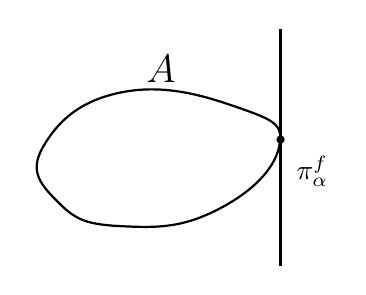
\begin{tikzpicture}
        % Dibujo del conjunto convexo A (forma irregular pero suave)
        \draw[thick] plot [smooth cycle, tension=0.8] coordinates {
            (0,0.5) (1,1.2) (2.5,1) (3,0.5) (2.2,-0.3) (1,-0.5) (0.2,-0.2)
        };
        
        % Etiqueta del conjunto A
        \node at (1.5,1.5) {\Large $A$};
        
        % Dibujo del hiperplano de soporte (línea vertical f = alpha)
        % El punto de contacto está aproximadamente en x = 3
        \draw[very thick] (3.02,-1) -- (3.02,2);
        
        % Etiqueta de la función de soporte f = alpha
        \node[right] at (3.1,0.2) {$\pi_\alpha^f$};
        
        % Punto de tangencia (opcional, para mayor precisión)
        \fill (3.02,0.6) circle (1.5pt);

    \end{tikzpicture}
    \caption{Ejemplo de un conjunto convexo $A$ y un hiperplano de soporte $\pi_\alpha^f$.}
    \label{fig:hiperplano-soporte}
\end{figure}


\begin{teo}[Teorema de Hahn-Banach fuerte]\label{teo:hahn-banach-fuerte}
    Sean $A, B$ conjuntos convexos no vacíos, con $A$ cerrado y $B$ compacto en un espacio normado $X$. Entonces existen $\alpha, \beta$ reales con $\alpha < \beta$ y $f \in X^*$ tales que
    \begin{equation*}
        f(a) \leq \alpha < \beta \leq f(b) \quad \forall a \in A, b \in B
    \end{equation*}
    Por lo tanto, el intervalo $(\alpha, \beta)$ separa los dos conjuntos.
\end{teo}

\section{Integración en espacios de Banach}

\begin{definicion}
    Sea $\varphi: [0, 1] \to X$ continua. Definimos la integral $\varphi$ en $X$ como el \tbf{único elemento} $y \in X$ tal que 
    $$f(y) = \int_{0}^{1} f \circ \varphi(t) dt \quad \forall f \in X^*$$
    En este caso lo llamamos 
    $$y := \int_{0}^{1} \varphi(t) dt$$
\end{definicion}


\begin{prop}
    Si $\varphi: [0, 1] \to X$ es continua, entonces 
    \begin{equation*}
        \left\| \int_{0}^{1} \varphi(t) dt \right\| \leq \int_{0}^{1} \|\varphi(t)\| dt
    \end{equation*}
\end{prop}


\noindent
En resumen la integral definida para funciones con valores en un espacio de Banach (a menudo llamada \tbf{integral de Bochner o de Riemann-Banach}) hereda las propiedades fundamentales del cálculo integral clásico de funciones reales, es decir, 

$$\int_{0}^{1} \varphi(t) dt$$
cumple
\begin{itemize}
    \item \tbf{Lineal respecto al integrando}:
    \begin{equation*}
        \int_{a}^{b} (\alpha \varphi(t) + \beta \psi(t)) \, dt = \alpha \int_{a}^{b} \varphi(t) \, dt + \beta \int_{a}^{b} \psi(t) \, dt, \quad \forall  \alpha,\beta\in \R, \varphi, \psi \text{ funciones},
    \end{equation*}
    \item \tbf{Teorema Fundamental del Cálculo(TFCI)}: si defines $G(x) = \int_{a}^{x} \varphi(t) \, dt$, entonces la derivada de esa función es el integrando: $G'(x) = \varphi(x)$. \\
    Si $\Phi$ es una primitiva de $\varphi$ (es decir, $\Phi' = \varphi$), entonces $\int_{a}^{b} \varphi(t) \, dt = \Phi(b) - \Phi(a)$.
    \item \tbf{Propiedad de la media}: podemos expresarlo de dos manera
    \begin{itemize}
        \item $\left\| \int_{a}^{b} \varphi(t) \, dt \right\| \leq \int_{a}^{b} \|\varphi(t)\| \, dt \leq (b-a) \sup\limits_{t \in [a,b]} \|\varphi(t)\|$
        \item El valor $\frac{1}{b-a} \int_{a}^{b} \varphi(t) \, dt$ pertenece a la clausura del casco convexo de la imagen de la función $\varphi([a,b])$.
    \end{itemize}
\end{itemize}

\chapter{Principio de Acotación Uniforme}

\begin{definicion}
    Sean $X, Y$ espacios normados y sea $\{T_\alpha\}_{\alpha \in A} \subseteq BL(X, Y)$. Se dice que $\{T_\alpha\}_{\alpha \in A}$ es \textbf{uniformemente acotada} si
    \begin{equation*}
        \exists M > 0 : \|T_\alpha\| \leq M \quad \forall \alpha \in A
    \end{equation*}
\end{definicion}

\begin{definicion}
    Sean $X, Y$ espacios normados y sea $\{T_\alpha\}_{\alpha \in A} \subseteq BL(X, Y)$. Se dice que $\{T_\alpha\}_{\alpha \in A}$ es \textbf{puntualmente acotada} si
    \begin{equation*}
        \forall x \in X : \{T_\alpha(x)\}_{\alpha \in A} \subseteq Y \text{ está acotada}
    \end{equation*}
\end{definicion}

\observacion{
    Si $\{T_\alpha\}$ está acotada uniformemente, entonces $\{T_\alpha\}$ está acotada puntualmente. De hecho:
    \begin{equation*}
        \|T_\alpha(x)\| \leq \|T_\alpha\| \cdot \|x\| \leq M \|x\| \implies \{T_\alpha(x)\} \subseteq Y \text{ está acotada}
    \end{equation*}
}

\begin{teo}[Teorema de Banach-Steinhaus o Principio de Acotación Uniforme]
    Sea $X$ un espacio de Banach e $Y$ un espacio normado, entonces toda familia $\{T_\alpha\}_{\alpha \in A} \subseteq BL(X, Y)$ puntualmente acotada es también uniformemente acotada. \\
    \noindent
    Es decir, si $\forall x \in X$ $\{T_\alpha(x)\}_{\alpha \in A} \subseteq Y$ está acotada, entonces 
    $$\exists M > 0 : \|T_\alpha\|_{BL(X, Y)} \leq M \quad \forall \alpha \in A$$
\end{teo}

\begin{notacion}
    Usualmente nos referiremos a este teorema por \tbf{PAU} o en inglés UBP (Uniform Boundedness Principle).
\end{notacion}

\begin{coro}
    Sea $X$ un espacio de Banach e $Y$ un espacio normado, si $\{T_n\}_{n \in \mathbb{N}} \subseteq BL(X, Y)$ converge puntualmente, es decir
    \begin{equation*}
        T_n(x) \longrightarrow T(x) \quad \forall x \in X \text{ en } Y
    \end{equation*}
    entonces $T$ es lineal y continuo.
\end{coro}

\begin{coro}
    Si $X$ es un espacio de Banach e $Y$ normado, entonces 
    $$BL(X, Y) \subseteq L(X, Y) = \{ T: X \to Y \text{ lineales} \}$$ 
    es cerrado.
\end{coro}


\subsection{Aplicaciones}

\begin{definicion}
    Una sucesión $(x_n)_{n\in \mathbb{N}}$ de un espacio normado $X$ es \textbf{infinitesimal} si $x_n \to 0$ en $X$.
\end{definicion}

\begin{coro}
    Sea $X$ un espacio normado y sea $B \subseteq X$, tenemos que
    \begin{equation*}
        \text{si } f(B)=\{f(x) \mid x \in B\} \text{ acotado } \forall f \in X^* \implies B \text{ está acotado}
    \end{equation*}
\end{coro}

\chapter{Teorema de la Aplicación Abierta}

\begin{coro}
    Una aplicación $f: X \longrightarrow Y$ es continua si y solo si la imagen inversa de cualquier abierto es un abierto. \\
    \noindent
    Es decir: si $V \subseteq Y$ es abierto $\implies f^{-1}(V) \subseteq X$ es abierto. \\
\end{coro}

\begin{definicion}
    Sean $X, Y$ espacios normados y $T: X \to Y$ una aplicación lineal. Se dice que $T$ es \textbf{abierta} si $T(A)$ es abierto para todo $A \subseteq X$ abierto. \\
\end{definicion}

\begin{teo}[Teorema de la aplicación abierta]
    Sean $X, Y$ espacios de Banach y $T \in BL(X, Y)$ sobreyectiva, entonces $T$ es abierta.
\end{teo}

\begin{coro}
    Sea $T\in BL(X, Y)$ con $X, Y$ espacios de Banach y $T$ biyectiva, entonces
    $$T^{-1} \in BL(Y, X)$$
\end{coro}

\begin{definicion}

    Sean $X, Y$ espacios topológicos, y $f$ una función de $X$ a $Y$; entonces, $f$ es un \tbf{homeomorfismo} si se cumple que:
    \begin{itemize}
        \item $f$ es una biyección
        \item $f$ es continua
        \item La inversa de $f$ es continua
    \end{itemize}
\end{definicion}

\subsection{Aplicaciones}
\noindent
Una de las aplicaciones más importantes del teorema de la aplicación abierta es la aproximación de soluciones de ecuaciones diferenciales. Queremos demostrar que si podemos aproximar una función ``difícil'' ($f$) mediante funciones ``fáciles'' (polinomios $p_n$), entonces las soluciones de la ecuación diferencial para esos polinomios ($x_n$) también aproximarán la solución real ($x$). \\ 


\begin{teo}[Teorema de Aproximación de Weierstrass]
    Si $f$ es una función real continua en $[a, b]$, entonces para cada $\epsilon > 0$, existe un polinomio $p$ tal que $|f(t) - p(t)| < \epsilon$ para todo $t \in [a, b]$. \\
    \noindent
    Esto equivale a decir, que el espacio de los polinomios es denso en $C^0([a, b])$ con la norma del supremo.
\end{teo}

\begin{coro}\label{coro:equivalencia-normas}
    Sea $X$ un espacio vectorial y sean $(X, \|\cdot\|_1)$, $(X, \|\cdot\|_2)$ espacios de Banach, y supongamos que $\exists M > 0 : \|x\|_2 \leq M \cdot \|x\|_1$, entonces
    \begin{equation*}
        (X, \|\cdot\|_1), (X, \|\cdot\|_2) \text{ son equivalentes}
    \end{equation*}
\end{coro}

\section{Teorema del Gráfico Cerrado}

\begin{definicion}
    Sea $T: X \to Y$ una aplicación entre espacios normados. Se dice que 
    \begin{equation*}
        \Gamma_T = \{ (x, T(x)) \mid x \in X \} \subseteq X \times Y
    \end{equation*}
    es el \tbf{gráfico} de $T$. \\
\end{definicion}

\begin{definicion}
    Sea $T: X \to Y$ con $X, Y$ espacios normados. Se dice que $T: X \to Y$ es \textbf{cerrado} si $\Gamma_T$ es cerrado en $X \times Y$. \\
\end{definicion}

\begin{prop}
    Sea $T: X \to Y$ una aplicación entre espacios normados, entonces
    \begin{equation*}
        \Gamma_T \text{ es cerrado en } X \times Y \iff \forall (x_n) \subseteq X : x_n \to x \text{ y } T(x_n) \to y, \text{ entonces } y = T(x)
    \end{equation*}
\end{prop}

\observacion{
    Si $T$ es continua, entonces $\Gamma_T$ es cerrado. De hecho
    \begin{equation*}
        \text{si } x_n \to x, \text{ entonces } T(x_n) \to T(x)
    \end{equation*}
    y por lo tanto $(x_n, T(x_n)) \to (x, T(x)) \quad \forall (x_n) \to x$. \\
}

\begin{teo}[Gráfico cerrado]
    Sean $X, Y$ espacios de Banach, tenemos que si
    \begin{equation*}
        T: X \to Y \text{ es lineal y cerrada } \implies T \text{ es continua}
    \end{equation*}
\end{teo}

\begin{coro}
    Sea $T: X \to Y$ lineal con $X, Y$ espacios de Banach, tenemos que si 
    \begin{equation*}
        T \text{ es cerrada y inyectiva} \implies T^{-1} \text{ continua}
    \end{equation*}
\end{coro}

\section{Ortogonalidad en espacios de Banach}

\noindent
En esta sección tomaremos $X$ un espacio de Banach, $M\subseteq X$ un subespacio de $X$ y $N\subseteq X^*$ un subespacio de $X^*$.

\begin{definicion}
    Se define el \tbf{ortogonal} de $M$ como el subespacio $M^{\perp} \subseteq X^*$ tal que
    \begin{equation*}
        M^{\perp} := \{ f \in X^* \mid f(x) = 0 \quad \forall x \in M \}
    \end{equation*}
    Se define el \tbf{ortogonal} de $N$ como el subespacio $N^{\perp} \subseteq X$ tal que
    \begin{equation*}        
        N^{\perp} := \{ x \in X \mid f(x) = 0 \quad \forall f \in N \}
    \end{equation*}
    $M^{\perp}$ y $N^{\perp}$ son llamados \tbf{aniquiladores}.
\end{definicion}

\observacion{
    $M^{\perp}$ y $N^{\perp}$ son \underline{subespacios cerrados} incluso si $M$ y $N$ no lo son.
}

\begin{prop}
    Sea $M\subseteq X, N \subseteq X^*$, se cumple:
    \begin{enumerate}
        \item[i)] $(M^{\perp})^{\perp} = \overline{M}$
        \item[ii)] $\overline{N} \subseteq (N^{\perp})^{\perp}$. Si $X$ es reflexivo, se cumple $(N^{\perp})^{\perp} = \overline{N}$
    \end{enumerate}
\end{prop}


\begin{prop}
    Sean $M_1, M_2$ subespacios de $X$, entonces
    \begin{enumerate}
        \item $M_1 \cap M_2 = (M_1^\perp + M_2^\perp)^\perp$
        \item $M_1^\perp \cap M_2^\perp = (M_1 + M_2)^\perp$
        \item $\overline{M_1^\perp + M_2^\perp} \subseteq (M_1 \cap M_2)^\perp$
        \item $(M_1^\perp \cap M_2^\perp)^\perp = \overline{M_1 + M_2}$
    \end{enumerate}
\end{prop}


\section{Operadores no acotados}

\begin{definicion}
    Sean $X,Y$ espacios de Banach y sea $D(T)$ un subespacio denso de $X$, un operador lineal $T$ definido como sigue
    \begin{equation*}
        T: D(T) \to Y
    \end{equation*}
    se dice \textbf{no acotado}.
\end{definicion}

\observacion{
    La definición extiende la definición de operador acotado porque $D(T)$ no es cerrado en general y, por lo tanto, no es necesariamente de Banach. 
}

\begin{observacion}
    En general, $T$ no envía acotados en acotados.
\end{observacion}

\begin{definicion}
    Dado $T: D(T) \to Y$ no acotado, si 
    
    \begin{equation*}
        \exists M > 0 \text{ tal que } \|T(x)\|_Y \leq M \cdot \|x\|_X \quad \forall x \in D(T)
    \end{equation*}
    entonces $T$ se dice \textbf{acotado} en $D(T)$.
\end{definicion}



\begin{definicion}
    Sea $T: D(T) \to Y$ no acotado, definimos los subespacios.
    \begin{itemize}
        \item $\text{Ker}(T) := \{ x \in D(T) \mid T(x) = 0 \}$
        \item $R(T) := \{ y \in Y \mid y = T(x) \text{ para algún } x \in D(T) \}$ (\tbf{rango})
    \end{itemize}
\end{definicion}

\begin{definicion}
    Sea $T: D(T) \to Y$ no acotado. $T$ se dice \tbf{densamente definido} en $X$ si $D(T)$ es denso en $X$. \\
\end{definicion}

\begin{prop}
    Si $T$ es cerrado, entonces $\text{Ker}(T)$ es cerrado.
\end{prop}

\subsection{Operador Adjunto}

\noindent
A continuación trabajaremos con el operador $T: D(T) \to Y$ densamente definido en $X$ y con $X, Y$ espacios de Banach, y usaremos el \underline{operador adjunto} $T^*$ definido en
\begin{equation*}
    D(T^*) = \{ g \in Y^* \mid \exists C > 0 \text{ tal que } |\langle g, T(u) \rangle| \le C \cdot \|u\| \quad \forall u \in D(T) \}
\end{equation*}
donde $\langle g, T(u) \rangle = g(T(u))$. \\

\begin{prop}
    Si el operador $T$ es acotado, entonces
    \begin{equation*}
        D(T^*) = Y^*
    \end{equation*}
\end{prop}

\noindent
Sea la siguiente función
\Func{f}{D(T)}{\mathbb{R}}{u}{\langle g, T(u) \rangle}
donde $g \in D(T^*)$, entonces $f$ es acotada, ya que 
\begin{equation*}
    |f(u)| = |\langle g, T(u) \rangle| \le C \cdot \|u\| \quad \forall u \in D(T)
\end{equation*}
Por hipótesis $D(T)$ es denso en $X$, para poder definir $T^*$, y además como $f$ es acotada, entonces $f$ puede ser extendida a $F \in X^*$, es decir
\begin{equation*}
    \exists F \in X^* : F(u) = f(u) = \langle g, T(u) \rangle \quad \forall u \in D(T)
\end{equation*}
Dada esta conclusión podemos definir correctamente el operador adjunto $T^*$ de $T$ de la siguiente manera, veámoslo. \\

\begin{definicion}
    Sea $T: D(T) \longrightarrow Y$ densamente definido en $X$ con $X, Y$ espacios de Banach. Definimos el \textbf{operador adjunto} $T^*$ de $T$ como el operador
    \Func{T^*}{D(T^*)}{X^*}{g}{T^*(g)=F}
    para el cual tenemos que 
    \begin{equation*}
        \langle T^*g, u \rangle = (T^*g)(u) = F(u) = f(u) = \langle g, T(u) \rangle \quad \forall u \in D(T), \forall g \in D(T^*) 
    \end{equation*}
    donde $D(T^*)$ es el subespacio de $Y^*$ definido por
    \begin{equation*}
        D(T^*):= \{ g \in Y^* \mid \exists C > 0 \text{ tal que } |\langle g, T(u) \rangle| \le C \cdot \|u\| \quad \forall u \in D(T) \}
    \end{equation*}
    donde $\langle g, T(u) \rangle = g(T(u))$. \\
\end{definicion}

\chapter{Convergencia débil}
\begin{definicion}
    Sea $X$ un espacio normado y $\{x_n\} \subseteq X$. Se dice que $x_n$ \textbf{converge débilmente} a $x \in X$ si
    \begin{equation*}
        F(x_n) \longrightarrow F(x) \quad \forall F \in X^*
    \end{equation*}
    y escribiremos $x_n \rightharpoonup x$. \\
\end{definicion}

\begin{observacion}
    Llamaremos \tbf{convergencia fuerte} a la convergencia habitual, es decir, $x_n \longrightarrow x$ si \mbox{$\|x_n - x\| \longrightarrow 0$}.
\end{observacion}

\begin{prop}
    El límite débil es único. \\
\end{prop}

\begin{prop}
    Si $x_n \longrightarrow x$ en $X$ (convergencia fuerte), entonces $x_n\rightharpoonup x$ (convergencia débil).
\end{prop}

\begin{prop}
    Sea $\{x_n\}$ una sucesión convergente débilmente a $x \in X$. Entonces $\{x_n\}$ es acotada y se cumple
    \begin{equation*}
        \|x\| \le \liminf_{n \to +\infty} \|x_n\| 
    \end{equation*} \\
\end{prop}


\begin{definicion}
    Sea $C\subseteq X$ se dice \tbf{débilmente cerrado} (por sucesiones) si para toda $\{x_n\} \subseteq C$ convergente débilmente a $x \in X$, entonces $x \in C$.
\end{definicion}

\begin{definicion}
    Sea $K\subseteq X$ se dice \tbf{débilmente compacto} (por sucesiones) o \tbf{débilmente secuancialmente compacto} si para toda $\{x_n\} \subseteq K$ existe una subsucesión convergente débilmente en $K$.
\end{definicion}

\begin{observacion}
    La \tbf{envolvente convexa} (o convex hull) de un conjunto de puntos $\{x_n\}$ es el conjunto más pequeño que contiene a todos esos puntos y que además es convexo. \\
\end{observacion}

\begin{teo}[Mazur]
    Sea $\{x_n\} \subseteq X$ tal que $x_n \rightharpoonup x_0$, entonces $x_0 \in \overline{Co(x_n)}$, donde:
    \begin{equation*}
        Co(x_n) := \text{envolvente convexa de } \{x_n\}
    \end{equation*}
\end{teo}

\begin{coro}
    Sea $C \subseteq X$ cerrado y convexo; entonces es débilmente cerrado.
\end{coro}

\observacion{
    Sea $X$ de dimensión finita, entonces la convergencia débil implica la convergencia fuerte. 
}

\begin{definicion}
    Sean $X, Y$ espacios normados de Banach, $T$ se dice \tbf{débilmente secuancialmente continuo} si para cada $\{x_n\} : x_n \rightharpoonup x$, entonces $T(x_n) \rightharpoonup T(x)$. \\
\end{definicion}

\begin{prop}
    Sea $T: X \longrightarrow Y$ lineal, entonces
    \begin{equation*}
        T \text{ es débilmente secuancialmente continuo} \iff T \text{ es continuo}
    \end{equation*}
\end{prop}

\begin{teo}[Eberlein]
    Si $X$ es un espacio reflexivo, entonces toda sucesión acotada admite una subsucesión débilmente convergente. \textit{\small(Los conjuntos acotados son débilmente secuencialmente compactos)}.
\end{teo}


\begin{coro}
    Sea $C$ cerrado, convexo y acotado en $X$, un espacio de Banach reflexivo. Entonces $C$ es débilmente secuencialmente compacto.
\end{coro}

\observacion{
    También vale el recíproco (difícil), es decir, si $C$ es débilmente secuancialmente compacto, entonces $C$ es acotado.
}

\begin{coro}
    Sea $X$ un espacio de Banach reflexivo y sea $C$ cerrado no vacío y convexo; entonces $C$ admite un punto de norma mínima.
\end{coro}

\begin{coro}
    Sea $C$ cerrado y convexo no vacío, entonces 
    $$\forall x \in X \quad \exists y \in C : \|x - y\| = \min_{z \in C} \|x - z\| = d(x, C)$$
\end{coro}

\section{Convergencia $*-$débil}
\noindent
Sea $X$ un espacio normado y sean $\{f_n\} \in X^*$, estudiamos la convergencia débil en $X^*$

\begin{equation*}
    f_n \rightharpoonup  f \text{ en } X^* \text{ si } G(f_n) \longrightarrow G(f) \quad \forall G \in X^{**}
\end{equation*}
donde $J: X \longrightarrow X^{**}$, $J_x(f) = f(x)$ no es sobreyectiva en general y $J(X) \subseteq X^{**}$.

\begin{definicion}
    Sea $\{f_n\} \subseteq X^*$, diremos que $f_n$ \textbf{converge *-débilmente} a $f \in X^*$ si
    \begin{equation*}
        J_x(f_n) \longrightarrow J_x(f) \quad \forall x \in X
    \end{equation*}
    es decir, $f_n(x) \longrightarrow f(x) \quad \forall x \in X$. Se nota como 
    \begin{equation*}
        f_n \overset{*}{\rightharpoonup} f \text{ en } X^*
    \end{equation*}
\end{definicion}

\observacion{
    El límite $*-$débil de $\{f_n\}$ es único, pues si $f_n \overset{*}{\rightharpoonup} f_1$ y $f_n \overset{*}{\rightharpoonup} f_2$, entonces \mbox{$f_n(x) \longrightarrow f_1(x)$} y \mbox{$f_n(x) \longrightarrow f_2(x)$} puntualmente para todo $x \in X$, por lo que $f_1(x) = f_2(x)$ para todo $x \in X$.
}

\observacion{
    Si $f_n \longrightarrow f$ en $X^*$ (convergencia fuerte), entonces $f_n \rightharpoonup f$ en $X^*$ (convergencia débil), entonces $f_n \overset{*}{\rightharpoonup} f$ en $X^*$. \\
}

\begin{prop}
    La convergencia fuerte implica la convergencia débil, y esta última implica la convergencia $*-$débil.
\end{prop}

\observacion{
    Si $X$ reflexivo, entonces
    \begin{equation*}
        f_n \rightharpoonup f \text{ en } X^* \iff f_n \overset{*}{\rightharpoonup} f \text{ en } X^*
    \end{equation*}
    Si $X$ no es reflexivo, entonces la convergencia débil y la convergencia $*-$débil en $X^*$ son diferentes. \\
}

\begin{teo}
    Sea $X$ un espacio de Banach separable. Toda sucesión de funcionales $\{f_n\} \subseteq X^*$ acotada en $X^*$ admite una subsucesión $*$-débilmente convergente.
\end{teo}

\observacion{
    Si $X$ no es seperable, en general no vale.
}

\begin{teo}[Teorema de Banach-Alaoglu]
    Sea $X$ un espacio de Banach, entonces $B^*$, la bola cerrada en $X^*$, es débilmente-* compacta.
\end{teo}

\observacion{
    En un espacio de Hilbert (lo veremos más adelante), la convergencia débil y la convergencia débil$-*$ son exactamente la misma cosa, pues $\mathcal{H}^* \cong \mathcal{H}$.
}

\begin{coro}
    Si $H$ es un espacio de Hilbert, la bola cerrada $B = \{x \in H : \|x\| \le 1\}$ es débilmente compacta. Por tanto, de cualquier sucesión acotada en $H$ se puede extraer una subsucesión débilmente convergente.
\end{coro}

\section{Espacios uniformemente convexos}

\begin{definicion}
    Un espacio normado $X$ se dice \textbf{estrictamente convexo} si
    \begin{equation*}
        \forall x, y \in X \text{ con } x \neq y, \|x\| = \|y\| = 1 \implies \left\| \frac{x+y}{2} \right\| < 1
    \end{equation*}
    \textit{\small (el punto medio de 2 vectores unitarios cae dentro de la bola)}
\end{definicion}

\begin{definicion}
    Un espacio normado $X$ se dice \tbf{uniformemente convexo} si 
    \begin{equation*}
        \forall \varepsilon > 0, \exists \delta > 0 \text{ tal que } \|x\|, \|y\| \leq 1, \|x - y\| \ge \varepsilon \implies \left\| \frac{x+y}{2} \right\| \leq 1 - \delta
    \end{equation*}
    \textit{\small (el punto medio de 2 vectores unitarios que están al menos $\varepsilon$ de distancia cae dentro de la bola cerrada de radio $1 - \delta$)}
\end{definicion}

\begin{lema}
    Sea $X$ un espacio de Banach, entonces
    \begin{equation*}
        X \text{ es reflexivo} \iff \forall F \in X^* \quad \exists x_0 \in X : \|x_0\| = 1 \text{ y } \|F\| = |F(x_0)|
    \end{equation*}
\end{lema}

\begin{teo}[Teorema de Milman-Pettis]
    Sea $X$ un espacio de Banach uniformemente convexo, entonces $X$ es reflexivo.
\end{teo}




\section{Topologías débiles}


\noindent
Sea $X$ un conjunto y sea $\{Y_i\}$ una familia de espacios topológicos tales que existen funciones $\varphi_i: X \to Y_i$ para todo $i$. \\

\noindent
Queremos dotar a $X$ de una topología $\mathcal{T}$ que haga continuas a las $\{\varphi_i\}$ y que sea la menos fina (más pequeña) con esta propiedad. Es decir

\begin{equation*}
    \forall W_i\subseteq Y_i \text{ abierto}, \varphi_i^{-1}(W_i) \text{ es abierto en } (X, \mathcal{T}) \text{ para todo } i
\end{equation*}
\noindent
Sea $\mathcal{F}$ una familia de subconjuntos de $X$ tal que la intersección finita $\bigcap\limits_{\text{finitas}} \varphi_i^{-1}(W_i)$ está contenida en $X$ y contiene la unión arbitraria $\bigcup \varphi_i^{-1}(W_i)$. \\ \\
\noindent
Después de haber realizado estas dos operaciones obtenemos que $\mathcal{F}$ es estable por intersecciones finitas y uniones, y contiene a $\varphi_i^{-1}(W_i)$ para todo $W_i$ abierto en $Y_i$ y para todo $i$; por construcción, es la topología más pequeña con estas propiedades. \\
\noindent
Definimos entonces $\mathcal{T} = \mathcal{F}$.


\begin{prop}
    Sea $x_0 \in X$ y sea $\{\bigcap\limits_{\text{finitas}} \varphi_i^{-1}(V_i)\}$ una base de entornos de $x_0$, donde cada $V_i$ es un entorno de $\varphi_i(x_0)$ en $Y_i$ para todo $i$. Entonces
    \begin{equation*}
        x_n \to x \text{ en } (X, \mathcal{T}) \iff \varphi_i(x_n) \to \varphi_i(x) \text{ en } Y_i \quad \forall i
    \end{equation*}
\end{prop}

\begin{definicion}
    Sea $X$ un espacio normado y $\mathcal{T}$ la topología menos fina que hace continuas las aplicaciones $F \in X^*$. Definimos $\mathcal{T}$ como la \textbf{topología débil}. \textit{\small (Es el caso precedente con $Y_i = \mathbb{R} \ \forall i$)} \\
\end{definicion}

\observacion{
    $(X, \|\cdot\|)$ hace continuas las aplicaciones de $X^*$ y, por lo tanto, también las de $(X, \mathcal{T})$.
    \[ x_m \xrightarrow{\mathcal{T}} x \text{ en } (X, \mathcal{T}) \iff F(x_m) \longrightarrow F(x) \text{ en } \mathbb{R} \ \forall F \in X^* \iff x_m \rightharpoonup x \]

}

\observacion{
    Sea $x_0 \in X$, una base de entornos se obtiene como
    \[ V_\varepsilon(x_0) = \{ x \in X \mid |F(x) - F(x_0)| < \varepsilon \ \forall F \text{ en un subconjunto finito de } X^* \} \]
}

\begin{prop}
    $(X, \mathcal{T})$ satisface el axioma de separación $T_2$ (Hausdorff). \\
\end{prop}

\observacion{
    En dimensión finita, la topología fuerte y la topología débil coinciden.
}

\begin{observacion}
    Cuando hacemos alusión a la topología fuerte en un espacio normado $(X,\|\cdot\|)$, nos referimos a la topología inducida por la norma $\|\cdot\|$ y, por lo tanto, a la convergencia fuerte. Por otro lado, cuando hablamos de la topología débil en $(X, \mathcal{T})$, nos referimos a la topología menos fina que hace continuas a las aplicaciones de $X^*$ y, por lo tanto, a la convergencia débil.
\end{observacion}

\observacion{
    Sea $(X, \|\cdot\|)$ un espacio normado de dimensión infinita, entonces $(X, \mathcal{T})$ débil es siempre estrictamente menos fina (más pequeña) que $(X, \|\cdot\|)$ con topología fuerte. En particular
    \begin{equation*}
        B = \{ x \in X \mid \|x\| < 1 \}
    \end{equation*}
    nunca es abierto en $(X, \mathcal{T})$, pues se puede ver que cada entorno de $x_0 \in (X, \mathcal{T})$ contiene una recta vectorial que pasa por $x_0$, por lo tanto, $B$ nunca es abierto. 
}

\observacion{
    En dimensión infinita, $(X, \|\cdot\|)$ nunca es metrizable. Existen espacios en los que la convergencia por sucesiones 
    $$x_m \to x \iff x_m \rightharpoonup x$$
    pero no es metrizable. 
}

\noindent
Intuitivamente, la topología débil tiene ``menos abiertos'' y, por lo tanto, ``más compactos'', entonces podemos minimizar funcionales sobre los compactos.

\chapter{Espacios de Hilbert}

\begin{definicion}
    Sea $X$ un espacio vectorial sobre $\mathbb{R}$. Se dice que $X$ es un \textbf{espacio con producto interno} si existe una aplicación:
    \Func{(\cdot, \cdot)}{X \times X}{\mathbb{R}}{(x,y)}{x\cdot y=(x,y)}
    tal que:
    \begin{itemize}
        \item[i)] $(x + y, z) = (x, z) + (y, z) \quad \forall x, y, z \in X$
        \item[ii)] $(\alpha x, y) = \alpha(x, y) \quad \forall x, y \in X, \ \forall \alpha \in \mathbb{R}$
        \item[iii)] $(x, y) = (y, x) \quad \forall x, y \in X$
        \item[iv)] $(x, x) \geq0$ \ y \ $(x, x) = 0 \iff x = 0 \quad \forall x \in X$
    \end{itemize}
    Sobre $\mathbb{C}$, la condición $iii)$ se sustituye por $iii)'$: $(x, y) = \overline{(y, x)}$ y por lo tanto:
        $$(x, \alpha y + \beta z) = \bar{\alpha}(x, y) + \bar{\beta}(x, z) \quad \forall \alpha, \beta \in \mathbb{C} \text{ \textit{(producto sesquilineal)}}$$
    Destacar que la diferencia con el producto interno en $\R$ es que esta vez el producto interno es lineal en la primera variable y conjugado lineal en la segunda.
\end{definicion}

\observacion{
    Las condiciones $i)$ y $ii)$ nos dicen que $(\cdot, \cdot)$ es lineal en la primera variable y, junto con $iii)$, se tiene que $(\cdot, \cdot)$ es bilineal sobre $\mathbb{R}$.
}

\begin{observacion}
    $(X, (\cdot, \cdot))$ es un espacio normado con norma $\|x\| := (x, x)^{1/2}$. \\
\end{observacion}

\begin{prop}[Desigualdad de Cauchy-Schwarz]
    Sea $X$ un espacio con producto interno, entonces se cumple:
    \[ |(x, y)| \le \|x\| \cdot \|y\| \quad \forall x, y \in X \]
\end{prop}

\begin{definicion}
    Un espacio $(X, (\cdot, \cdot))$ con producto interno se dice \textbf{espacio de Hilbert} \mbox{$\mathcal{H} = (X, (\cdot, \cdot))$} si es completo.
\end{definicion}

\begin{ejemplo}
    \begin{itemize}
        \item $\ell_2$ es un espacio de Hilbert
        $$(x, y) := \sum_{k=0}^{+\infty} x_k \cdot \overline{y_k}$$
        \item $L^2(A)$ es un espacio de Hilbert
        $$(f, g) := \int_A f \bar{g} \, d\mu$$
    \end{itemize}
\end{ejemplo}


\noindent
Buscamos un criterio que nos permita entender cuándo un espacio normado tiene una norma que deriva de un producto interno.

\begin{teo}[Ley del paralelogramo]\label{teo:paralelogramo}
    Sea $(X, \|\cdot\|)$ un espacio normado, entonces
    \begin{equation*}
        X \text{ espacio con producto interno con } \|x\|^2 := (x, x) \iff \|x+y\|^2 + \|x-y\|^2 = 2\|x\|^2 + 2\|y\|^2 \quad \forall x, y \in X
    \end{equation*}
\end{teo}

\begin{prop}
    $z = 0 \iff (x, z) = 0 \quad \forall x \in X$\\
\end{prop}

\observacion{
    Sea $\bar{x}\in X$ tal que $F_{\bar{x}}(y) = (\bar{x}, y) \quad \forall y \in Y$, entonces $F_{\bar{x}}$ es lineal y continuo.
}

\begin{teo}
    Todo espacio con producto interno $(X, (\cdot, \cdot))$ es uniformemente convexo. \\
\end{teo}

\begin{teo}[Teorema de proyección]
    Sea $\mathcal{H}$ un espacio de Hilbert, y sea $C \subseteq \mathcal{H}$ un subconjunto no vacío, cerrado y convexo, entonces para cada $x \in \mathcal{H}$ existe un único $x_0 \in C$ tal que:
    \[ \|x - x_0\| = \inf_{y \in C} \|x - y\| \]
    Además, $x_0$ está caracterizado por la siguiente propiedad
    \begin{equation*}
        x_0 \text{ es el único punto de } C \text{ tal que } (x - x_0, y - x_0) \le 0 \quad \forall y \in C
    \end{equation*}
    El punto $x_0 \in X$ se denomina proyección de $x$ sobre $C$ y se indica como $P_C(x)$.
\end{teo}


\section{Ortogonalidad en espacios de Hilbert}

\begin{definicion}
    Sean $x, y \in \mathcal{H}$, se dice que $x$ es \textbf{ortogonal} a $y$ si $(x, y) = 0$, y escribiremos $x \perp y$.
\end{definicion}

\begin{prop}
    Si $x \perp y$, entonces se tiene 
    \begin{itemize}
        \item[i)] $y \perp x$
        \item[ii)] $x \perp (-y)$
        \item[iii)] $x \perp x \iff x = 0$
    \end{itemize}
\end{prop}

\begin{definicion}
    Sean $A, B \subseteq \mathcal{H}$ subconjuntos. Se dice que $x \in \mathcal{H}$ es \textbf{ortogonal a $A$} ($x \perp A$) si 
    $$(x, a) = 0 \quad \forall a \in A$$ 
    \noindent
    Se dice que $A$ es \textbf{ortogonal a $B$} ($A \perp B$) si 
    $$(a, b) = 0 \quad \forall a \in A, \ \forall b \in B$$ 
    \noindent
    El \textbf{conjunto ortogonal a $A$} se define como:
    \[ A^\perp := \{ x \in \mathcal{H} \mid (x, a) = 0 \quad \forall a \in A \} \]
\end{definicion}

\begin{prop}\label{prop:ortogonalidad}
    Se cumplen las siguientes propiedades:
    \begin{enumerate}
        \item $0^{\perp} = \mathcal{H}$ \ y \ $\mathcal{H}^{\perp} = \{0\}$
        \item $A \cap A^{\perp} \subseteq \{0\}$
        \item (\textit{Teorema de Pitágoras}) si $x \perp y$ entonces $\|x + y\|^2 = \|x\|^2 + \|y\|^2$
        \item Sean $A, B$ subconjuntos con $A \subseteq B$ entonces $B^{\perp}\subseteq A^{\perp}$
    \end{enumerate}
\end{prop}

\begin{prop}
    Sea $x \in \mathcal{H}$ y sea $x_0 := P_{M}(x)$, donde $M\subseteq\mathcal{H}$ no vacío, cerrado y convexo, entonces $x_0$ está caracterizado por estas dos condiciones
    \begin{itemize}
        \item[i)] $x_0 \in M$
        \item[ii)] $(x - x_0, y) = 0 \quad \forall y \in M \quad (x - x_0 \in M^\perp)$.
    \end{itemize}
    es decir, $x_0=P_M(x)$ si y solo si se cumplen $i)$ y $ii)$. \\
    \noindent
    Además, la función $P_M$
    \Func{P_M}{\mathcal{H}}{M}{x}{P_M(x)}
    es un operador lineal y continuo, y se define como \textbf{proyección ortogonal sobre $M$}. \\
\end{prop}

\begin{definicion}
    Sea $X$ un espacio normado, $X$ es la \textbf{suma directa} de dos subespacios $A, B$ si
    \begin{itemize}
        \item $A, B$ son cerrados.
        \item $A \cap B = \{0\}$
        \item $A + B = X$
    \end{itemize}
    y diremos $X = A \oplus B$.
\end{definicion}

\begin{teo}[Teorema de descomposición ortogonal]
    Sea $M$ un subespacio cerrado, entonces 
    $$\mathcal{H} = M \oplus M^\perp$$
\end{teo}


\observacion{
    Si $\mathcal{H} = M \oplus M^\perp$, la descomposición es única, veámoslo. Si $x = \overbrace{a}^{\in M} + \overbrace{b}^{\in M^\perp}$, entonces 
    $$x - a = b \in M^\perp \implies (x - a, y) = 0 \quad \forall y \in M \implies a = P_M(x) = x_0 \text{ y } b = x - x_0$$
    tenemos por tanto que $a=x_0$ es único y $b = x - x_0$ también es único, por la noción de que la proyección de $x$, es decir, $x_0$, es única.
}

\observacion{
    Sea $A \subseteq \mathcal{H}$ un subespacio, entonces se cumple:
    \begin{itemize}
        \item[i)] $A \subseteq (A^\perp)^\perp$
        \item[ii)] $(A^\perp)^\perp = \overline{A}$. En particular si $A$ es cerrado, entonces $A = (A^\perp)^\perp$
    \end{itemize}
}

\observacion{
    Sea $X$ un espacio con producto interno y sea 
    \Func{T}{X}{X^*}{y}{F_y}
    donde $F_y(x) = (x, y) \quad \forall x \in X$, entonces $T$ es inyectiva e isometría. \\ \\
}

\begin{teo}[Teorema de Riesz]
    Sea $\mathcal{H}$ un espacio de Hilbert, entonces 
    \begin{equation*}
        \forall F \in \mathcal{H}^* \quad \exists! y_F \in \mathcal{H} \text{ tal que } F(x) = (x, y_F) \quad \forall x \in \mathcal{H}
    \end{equation*}
    es decir, $T$ es sobreyectiva.
\end{teo}
\observacion{
    Hemos visto que $T: \mathcal{H} \longrightarrow \mathcal{H}^*$ es un isomorfismo algebraico y topológico (dijimos $T$ isometría, que implica acotación y de su inversa, y biyectiva), entonces $\mathcal{H}^*$ es un espacio de Hilbert.
}

\section{Operador adjunto}
\begin{definicion}
    Sea $T \in BL(\mathcal{H})$, se define como \textbf{operador adjunto} de $T$ a la aplicación
    \Func{T^*}{\mathcal{H}}{\mathcal{H}}{x}{T^*(x)}
    tal que $T^*(x)$ es el único vector que representa a $G_x$, es decir
    \[ G_x(y)=(x, T(y)) = (T^*(x), y) \quad \forall x, y \in \mathcal{H} \]
\end{definicion}

\begin{prop}
    Sea $T\in BL(\mathcal{H})$, entonces 
    \begin{itemize}
        \item[i)] $T^{**} = T$
        \item[ii)] $\|T^*\| = \|T\|$, y por lo tanto $T^* \in BL(\mathcal{H})$
    \end{itemize}
\end{prop}

\begin{prop}
    Sean $S, T \in BL(\mathcal{H})$, entonces se tiene:
    \begin{itemize}
        \item $(S + T)^* = S^* + T^*$
        \item $(\alpha T)^* = \bar{\alpha} T^*$
        \item $(S \circ T)^* = T^* \circ S^*$
        \item $\|T^* \circ T\| = \|T \circ T^*\| = \|T\|^2$ \\
    \end{itemize}
\end{prop}

\begin{definicion}
    Sea $T \in BL(\mathcal{H})$ se dice \textbf{autoadjunto} si $T = T^*$, es decir
    \[ (x, T(y)) = (T(x), y) \quad \forall x, y \in \mathcal{H} \]
\end{definicion}

\begin{teo}
    Sea $T \in BL(\mathcal{H})$ autoadjunto, entonces 
    \begin{equation*}
        \|T\| = \sup_{x \neq 0} \frac{|(T(x), x)|}{\|x\|^2} = \sup_{\|x\|=1} |(T(x), x)|
    \end{equation*}
\end{teo}

\begin{prop}
    Sea $T\in BL(\mathcal{H})$, entonces 
    \begin{equation*}
        T \text{ biyectivo} \iff T^* \text{ biyectivo}
    \end{equation*} 
\end{prop}

\section{Operadores compactos}

\begin{definicion}
    Sea $X$ un espacio normado, un subconjunto $K \subseteq X$ es \textbf{compacto} si toda sucesión $\{x_n\}$ en $K$ admite una subsucesión convergente a un punto de $K$. \\
\end{definicion}

\begin{definicion}
    Sea $X$ un espacio normado, un subconjunto $A \subseteq X$ es \textbf{relativamente compacto} si la clausura de $A$ es compacta. \\
\end{definicion}

\begin{definicion}
    Sean $X, Y$ espacios de Banach y sea $T\in BL(X,Y)$. $T$ se dice \textbf{operador compacto} si $T(C)$ es \underline{relativamente compacto} para cada conjunto $C$ acotado. \\
    \noindent
    Análogamente, $T$ es \tbf{operador compacto} si para cada $\{x_n\}$ sucesión acotada, $T(x_n)$ admite una subsucesión convergente. \\
\end{definicion}

\begin{ejemplo}
    \begin{enumerate}
        \item Si $T: X \to Y$ es lineal y $X, Y$ son espacios normados de dimensión finita, entonces $T$ es compacto.
        \item $Id: X \to X$ nunca es compacto para cualquier $X$ espacio normado de dimensión infinita. De hecho: la bola unitaria no es compacta.
    \end{enumerate}
\end{ejemplo}

\observacion{
    $\mathcal{K}(X, Y) := \{ T \in BL(X, Y) \text{ compacto} \} \subseteq BL(X, Y)$ es un subespacio de $BL(X, Y)$. \\
}

\begin{teo}
    Sea $\{T_n\} \subseteq \mathcal{K}(X, Y)$ una sucesión de operadores compactos tales que $T_n \to T\in BL(X, Y)$, entonces $T$ es compacto.
\end{teo}

\begin{prop}
    Sean $X$ un espacio de Banach e $Y$ un espacio de Hilbert, y sea $T \in K(X, Y)$. Entonces $T$ es el límite de $(T_n)_n$, donde $(T_n)_n$ es una sucesión de operadores con $R(T_n)$ de dimensión finita.
\end{prop}

\chapter{Sistemas ortonormales completos}

\begin{definicion}
    Sea $S\subseteq \mathcal{H}$ se dice \tbf{sistema ortonormal} si está constituido por vectores mutuamente ortogonales y de norma unitaria:
    \[ S = \{ e_i \in \mathcal{H}, \ i \in \mathcal{I} : (e_i, e_j) = \delta_{ij}\}\]
\end{definicion}



\observacion{
    Si $S$ es un sistema ortonormal, entonces $S$ es un sistema de vectores linealmente independientes.
}

\observacion{
    Si $S$ es un sistema de vectores linealmente independientes, entonces se puede construir una sucesión ortonormal mediante el proceso de \textbf{Gram-Schmidt}. \\
}

\begin{definicion}
    Un sistema ortonormal se dice \textbf{completo} si no está contenido propiamente en ningún otro sistema ortonormal (es decir, es maximal por inclusión). \\
\end{definicion}

\begin{prop}
    Sea $\mathcal{H}$ un espacio con producto interno, entonces por el \textbf{Lema de Zorn} siempre existe un sistema ortonormal completo. 
\end{prop}

\begin{coro}
        Sea $\mathcal{H}$ un espacio de Hilbert, entonces 
    \begin{equation*}
        S \text{ es un sistema ortonormal completo} \iff \text{ si } \forall x \in \mathcal{H}, x \perp S \text{ entonces } x = 0
    \end{equation*} \\
\end{coro}
\begin{prop}[Desigualdad de Bessel finita]
    Sea $\{e_i\}_{i=1}^{n}$ un sistema ortonormal en $\mathcal{H}$. Entonces, $\forall x \in \mathcal{H}$:
    \[ \sum_{i=1}^{n} (x, e_i)^2 \le \|x\|^2 \]
    Además, 
    $$x - \sum_{i=1}^{n} (x, e_i)e_i \perp e_j \quad \forall j=1, \dots, n$$
\end{prop}

\begin{prop}
    Sea $\mathcal{H}$ un espacio de Hilbert y sea $S = \{e_i\}_{i \in \mathcal{I}}$ un sistema ortonormal. Entonces, para cada $x \in \mathcal{H}$:
    \[ S(x) := \{ i \in \mathcal{I} \mid (x, e_i) \neq 0 \} \text{ es a lo sumo numerable} \]
\end{prop}

\begin{definicion}
    Sea $S \subseteq \mathcal{H}$ un sistema ortonormal completo, dado por $S = \{e_i\}_{i \in \mathcal{I}}$, entonces para cada $x \in \mathcal{H}$, definimos la serie:
    \[ \sum_{i \in \mathcal{I}} |(x, e_i)|^2 \quad \text{con } (x, e_i) := \text{coeficientes de Fourier de } x \text{ respecto a } S \]

\end{definicion}

\observacion{
    Si demostramos que $\sum_{i \in \mathcal{I}} |(x, e_i)|^2$ converge, entonces converge absolutamente y, por lo tanto, podemos permutar los índices.
}

\begin{teo}[Desigualdad de Bessel]
    Sea $S = \{e_i\}_{i \in \mathcal{I}}$ un sistema ortonormal, entonces para cada $x \in \mathcal{H}$: 
    \[ \sum_{i \in \mathcal{I}} |(x, e_i)|^2 \le \|x\|^2 \]
\end{teo}

\begin{definicion}
    Sea $S$ un sistema ortonormal en un espacio de Hilbert $\mathcal{H}$, entonces $\forall x \in \mathcal{H}$ está definida la suma de la serie:
    \[ \sum_{i \in \mathcal{I}} (x, e_i) e_i \quad \text{denominada \textbf{Serie de Fourier} de } x \text{ en } \mathcal{H} \]

\end{definicion}

\begin{prop}
    Sea $S$ un sistema ortonormal, entonces son equivalentes:
    \begin{enumerate}
        \item $S$ es completo.
        \item Si $x \in \mathcal{H}$ y $(x, e_i) = 0 \quad \forall i \in \mathcal{I} \implies x = 0$.
        \item Para cada $x \in \mathcal{H}$ se cumple
        $$x = \sum_{i \in \mathcal{I}} (x, e_i) e_i$$
        \item (\textbf{Identidad de Parseval}) Para cada $x \in \mathcal{H}$
        $$\|x\|^2 = \sum_{i \in \mathcal{I}} |(x, e_i)|^2$$
    \end{enumerate}
\end{prop}

\begin{teo} 
    Sea $\mathcal{H}$ un espacio de Hilbert, entonces
    \begin{equation*}
        \mathcal{H} \text{ es separable} \iff \text{ existe un sistema ortonormal } S \text{ completo y numerable}
    \end{equation*}
\end{teo}

\begin{teo}[Teorema isomorfismo euclídeo]
    Todo espacio de Hilbert $\mathcal{H}$ separable es isomorfo a $\ell_2$ mediante una isometría.
\end{teo}

\chapter{Teoría espectral}

\noindent 
Sea $F: X \to X$ una aplicación lineal y continua en un espacio de Banach $X$, entonces hemos visto que si $F$ es biyectiva, entonces $F^{-1}$ es continua. Sea 
$$F := T - \lambda Id$$
con $T \in BL(X)$, preguntémonos cuándo $F$ es biyectiva. \\

\begin{definicion}[Resolvente]
    Sea $T \in BL(X)$, definimos 
    $$\rho(T) := \{ \lambda \in \mathbb{R} \mid T - \lambda Id \text{ es biyectiva} \}$$
    como el \tbf{resolvente}.
\end{definicion}
\begin{definicion}[Espectro]
    Sea $T \in BL(X)$, definimos 
    $$\sigma(T) := \{ \lambda \in \mathbb{R} \mid T - \lambda Id \text{ no es biyectiva} \}=\R\setminus \rho(T)$$ 
    como el \tbf{espectro}. \\
\end{definicion}

\observacion{
    Si $\lambda \in \sigma(T)$, entonces $T - \lambda Id$ o no es inyectiva o no es sobreyectiva.
}

\begin{definicion}
    Sea $T\in BL(X)$, entonces $\lambda \in \sigma(T)$ se dice \textbf{valor propio} de $T$ si $T - \lambda Id$ no es inyectiva. Definimos 
    $$e(T) := \{ \lambda \in \sigma(T) \mid \lambda \text{ es valor propio} \} \subseteq \sigma(T)$$
    como el \tbf{conjunto de los valores propios}.
\end{definicion}

\observacion{
    Para el conjunto de valores propios tenemos estas propiedades
    \begin{itemize}
        \item $\lambda \in e(T) \iff \exists y \neq 0 : T(y) = \lambda y$ (ecuación de valores propios).
        \item $\lambda \in e(T) \iff \text{Ker}(T - \lambda Id) \neq \{0\}$.
    \end{itemize}
    En este caso, $y$ se llama \textbf{vector propio} de $T$ respecto a $\lambda$ y $\text{Ker}(T - \lambda Id)$ se llama \textbf{espacio propio} de $\lambda$, el cual es un subespacio cerrado.
}

\begin{teo}
    Sea $X$ un espacio de Banach y sea $T \in BL(X, Y)$, entonces
    \begin{enumerate}
        \item Si $\lambda_1, \lambda_2 \in e(T)$ con $\lambda_1 \neq \lambda_2\implies \text{Ker}(T - \lambda_1 I) \cap \text{Ker}(T - \lambda_2 I) = \{0\}$.
        \item Si $\{v_1, \dots, v_m\}$ son vectores propios correspondientes a valores propios distintos \mbox{$\lambda_1, \dots, \lambda_m \in e(T)$}, entonces $\{v_1, \dots, v_m\}$ es un conjunto de vectores linealmente independientes.
    \end{enumerate}
\end{teo}

\begin{teo}
    Sea $X$ un espacio de Banach y sea $T \in BL(X, Y)$, entonces
    \begin{enumerate}
        \item $\rho(T)$ es abierto.
        \item $\sigma(T) \subseteq [-\|T\|, \|T\|]$.
    \end{enumerate}
    De lo cual $\sigma(T)$ es compacto.
\end{teo}


\section{Operadores sobre los complejos}

\noindent 
Sea $T: H \to H$ un operador sobre $H$, un $\mathbb{C}$-espacio de Hilbert, entonces:
\begin{enumerate}
    \item[i)] Si $T$ es autoadjunto: $(T(x), x) = (x, T(x)) = \overline{(T(x), x)} \quad \forall x \in H \implies (T(x), x) \in \mathbb{R}$. \\
\end{enumerate}

\noindent 
Sea $X$ un espacio de Banach sobre $\mathbb{C}$ y $T \in BL(X)$. Definimos:
\[ \rho(T) := \{ \lambda \in \mathbb{C} \mid T - \lambda Id \text{ es biyectiva} \}, \quad \sigma(T) := \mathbb{C} \setminus \rho(T) \]

\begin{prop}
    Sea $T\in BL(\mathcal{X})$ con $X$ un espacio de Banach sobre $\mathbb{C}$, entonces \begin{enumerate}
        \item $\rho(T)$ es abierto en $\mathbb{C}$.
        \item $\sigma(T) \subseteq \{ \lambda \in \mathbb{C} \mid |\lambda| \leq \|T\| \}$, de lo cual $\sigma(T)$ es compacto.
    \end{enumerate}
\end{prop}

\begin{definicion}
    Definimos el \textbf{radio espectral} como  
    $$r(T) := \inf \{ r \geq 0 \mid \sigma(T) \subseteq B_r(0) \}$$
    y se llama \textbf{conjunto de valores propios} de $T$ a lo siguiente
    $$e(T) = \{ \lambda \in \sigma(T) \mid T - \lambda Id \text{ no es inyectiva} \}$$    
    Si $\lambda \in e(T)$, entonces $\dim(\text{Ker}(T - \lambda Id))$ se llama \textbf{multiplicidad geométrica} de $\lambda$.
\end{definicion}

\begin{teo}
    Sea $T \in BL(X)$, con $X$ espacio de Banach sobre $\mathbb{C}$, entonces 
    $$\sigma(T) \neq \emptyset$$
\end{teo}

\begin{teo}
    Sea $T$ un operador compacto, entonces 
    $$\text{Ker}(T - \lambda Id)$$
    es de dimensión finita $\forall \lambda \neq 0$.
\end{teo}

\begin{prop}
    Tenemos que
    \begin{equation*}
        \lambda \in \sigma(T) \iff \bar{\lambda} \in \sigma(T^*)
    \end{equation*}
\end{prop}

\begin{prop}
    Si $X$ es de dimensión infinita y $T \in K(X)$, entonces 
    $$0 \in \sigma(T)$$
\end{prop}

\begin{teo}
    Sea $T \in K(X)$, entonces
    \begin{enumerate}
        \item[i)] $e(T)$ es a lo sumo numerable.
        \item[ii)] Si $e(T)$ no es finito, entonces $0$ es el único punto de acumulación.
    \end{enumerate}
\end{teo}

\observacion{
    Si $T$ es compacto, $X$ es de Banach y  $e(T) = \{\lambda_m\}_m$ es numerable entonces 
    \begin{equation*}
            e(T) \subseteq [-\|T\|, \|T\|] \implies (\lambda_m) \text{ es acotada con } 0 \text{ como punto de acumulación} \implies \lambda_m \to 0 \\
    \end{equation*}
}

\begin{teo}[Teorema de la alternativa de Fredholm] \label{teo:fredholm}
    Sea $H$ un espacio de Hilbert y $T \in BL(H)$ compacto. Entonces:
    \begin{enumerate}
        \item[a)] si $\lambda \neq 0$, entonces $R(T - \lambda I)$ es cerrado y se cumple $R(T - \lambda I) = \text{Ker}(T^* - \bar{\lambda} I)^\perp$
        \item[b)] si $\lambda \neq 0$, entonces $\text{Ker}(T - \lambda I) = \{0\} \iff R(T - \lambda I) = H$, es decir:
        \[ T - \lambda I \text{ es inyectivo} \iff T - \lambda I \text{ es sobreyectivo} \]
        \item[c)] $\dim \text{Ker}(T - \lambda I) = \dim \text{Ker}(T^* - \bar{\lambda} I)$
    \end{enumerate}
\end{teo}

\begin{coro}
    Dado un operador
    \Func{T}{H}{H}{u}{T(u)}
    compacto, y $T\in BL(\mathcal{H})$, con $\mathcal{H}$ un espacio de hilbert de dimensión infinita tenemos que 
    \begin{itemize}
        \item $0 \in \sigma(T)$ (sea valor propio o no).
        \item $\sigma(T) \setminus \{0\} = e(T) \setminus \{0\}$ (apartado $b)$ del Teorema \ref{teo:fredholm}).
        \item Se tiene una de las siguientes alternativas:
        \begin{itemize}
            \item $\sigma(T) = \{0\}$
            \item $\sigma(T) \setminus \{0\} = e(T) \setminus \{0\}$ es un conjunto finito.
            \item $\sigma(T) \setminus \{0\} = e(T) \setminus \{0\}$ es una sucesión $\lambda_n$ que tiene a $\{0\}$ como único punto de acumulación y $\lambda_n \to 0$.
        \end{itemize}
    \end{itemize}
\end{coro}
\observacion{
    Para el caso $X$ un espacio de Banach y no de Hilbert, tenemos que también se cumple para $T$ compacto, lineal y continuo, que
    \begin{equation*}
        \sigma(T) \setminus \{0\} = e(T) \setminus \{0\}
    \end{equation*}
}

\section{Operadores autoadjuntos}
\begin{teo}
    Sea $T \in BL(H)$, $H$ espacio de Hilbert  y $T$ autoadjunto, definimos
    \begin{equation*}
        m := \inf_{\substack{u \in H \\ \|u\|=1}} (T(u), u ) \quad \text{y} \quad M := \sup_{\substack{u \in H \\ \|u\|=1}} ( T(u), u )
    \end{equation*}
    tenemos entonces que 
    \begin{equation*}
        \sigma(T) \subseteq [m, M] \quad \text{y} \quad m, M \in \sigma(T)
    \end{equation*}
\end{teo}


\observacion{
    Sabemos que $m\in \sigma(T)$, de hecho si $m$ fuera un valor propio (\tbf{no nulo}), entonces \underline{$m = \min$}. º\\
    \noindent
    Analógamente, si $M$ es un valor propio (\tbf{no nulo}), entonces \underline{$M = \max$}.
}

\begin{observacion}
    Es importante notar que los vectores propios no tienen porque ser unitarios, es decir, podemos obtener un vector propio $u\in \mathcal{H}$ con norma distinta de $1$, pero como el operador es lineal, entonces 
    $$T(u) = T\left(\|u\| \cdot \frac{u}{\|u\|}\right) = \|u\| \cdot T\left(\frac{u}{\|u\|}\right)$$
    por lo que $\frac{u}{\|u\|}$ también es un vector propio asociado al mismo valor propio. \\ \\
    \noindent
    Por lo tanto, sin pérdida de generalidad, podemos asumir que los vectores propios tienen norma $1$, ya que la clave radica en que las soluciones de la ecuación de autovalores no son vectores aislados, sino subespacios vectoriales completos (líneas, planos, etc.), por lo que no existe un vector propio único, sino que existe una infinidad de vectores propios asociados a un mismo valor propio, y entre ellos se encuentra uno con norma $1$.\\
\end{observacion}

\begin{coro}
    Sea $T$ autoadjunto, entonces tenemos que 
    \begin{equation*}
        \sigma(T)=\{0\}\implies T \equiv 0
    \end{equation*}
\end{coro}

\begin{prop}
    Sea $T \in BL(\mathcal{H})$ autoadjunto, entonces:
    \begin{itemize}
        \item $\sigma(T) =\{0\}\iff T\equiv 0$.
        \item $\sigma(T) \subseteq \mathbb{R}$.
        \item Si $\lambda_1, \lambda_2 \in \sigma(T)$ con $\lambda_1 \neq \lambda_2$, entonces los espacios propios correspondientes a $\lambda_1$ y $\lambda_2$ son ortogonales entre sí. \\
    \end{itemize}
\end{prop}

\begin{coro}
    Dado un operador $T\in BL(\mathcal{H})$ autodajunto y compacto, tenemos que \underline{existe al menos} \underline{un valor propio $\lambda$ tal que $|\lambda|=\|T\|$}, de hecho tenemos que
    \begin{itemize}
        \item $m = M = 0 \implies \sigma(T) = \{0\} \implies T \equiv 0$, no nos vale este caso.
        \item $m = 0, \ M > 0 \implies M$ es un valor propio y $M = \|T\|$ (por la caracterización de la norma de los op. autoadjuntos).
        \item $m < 0, \ M = 0 \implies m$ es un valor propio y $|m| = \|T\|$
        \item $m \neq 0, \ M \neq 0 \implies m$ y $M$ son valores propios y $\|T\| = \max\{|m|, |M|\}$.
    \end{itemize}
\end{coro}


\begin{teo}
    Sea $H$ espacio de Hilbert separable, $T \in BL(\mathcal{H})$ autoadjunto y compacto. Entonces existe una base hilbertiana, es decir, un sistema ortonormal completo formado por vectores propios de $T$.
\end{teo}


\begin{observacion}
    El teorema anterior es un resultado muy importante, porque nos dice que en este caso, el operador $T$ se puede diagonalizar completamente, es decir, se puede representar como una matriz diagonal con los valores propios en la diagonal y los vectores propios como columnas. Esto es análogo a lo que ocurre con las matrices simétricas en espacios finitos, pero en este caso estamos trabajando con operadores en espacios de Hilbert de dimensión infinita. \\
\end{observacion}

\begin{teo}
    Sea $X$ un espacio de Banach sobre $\C$ y $T \in BL(X)$, entonces 
    $$\sigma(T) \neq \emptyset$$
\end{teo}
\observacion{   
    Sea $\mathcal{H}$ espacio de Hilbert de dimensión infinita, observamos que dependiendo de si $0$ es valor o no propio, tenemos una cantidad de valores propios u otra, véamoslo:
    \begin{itemize}
        \item Si $0$ no es un valor propio, entonces $e(T)$ es numerable.
        \item Si $0$ es un valor propio de multiplicidad finita, entonces $e(T)$ es numerable.
        \item Si $0$ es un valor propio de multiplicidad geométrica infinita, entonces $e(T)$ puede ser finito.
    \end{itemize}
}
\begin{prop}
    Todo operador autoadjunto y compacto $T\in BL(\mathcal{H})$ se aproxima con operadores con imagen de dimensión finita.
\end{prop}

\section{Formulación variacional}

\noindent
En esta sección trabajaremos con $\mathcal{H}$ un espacio de Hilbert separable, $T\in BL(\mathcal{H})$ un operador autoadjunto y compacto. \\ \\
\noindent
Al tener $T$ autoadjunto y compacto, sabemos que los valores propios son reales y por tanto tienen signo: o son mayores o iguales que cero ($\geq 0$), o son menores o iguales que cero ($\leq 0$). Gracias a que \underline{no se pueden acumular en ningún otro sitio que no sea el origen} (Teorema \ref{teo:fredholm}), la matemática nos da permiso para hacer algo imposible en otros conjuntos de números reales: podemos hacer una fila india ordenada con ellos. \\
\noindent
Vamos a hacer dos listas ordenadas:
\begin{itemize}
    \item La lista de los positivos ($\lambda_m^+$): Se ordenan de mayor a menor (decreciente) marchando hacia el cero: $\lambda_1^+ \geq \lambda_2^+ \geq \dots \geq 0$.
    \item La lista de los negativos ($\lambda_m^-$): Se ordenan de menor a mayor (creciente, es decir, de los más negativos a los que se acercan al cero): $\lambda_1^- \leq \lambda_2^- \leq \dots \leq 0$.
\end{itemize}
Un punto crítico a tener en cuenta es que \textit{repitiremos cada valor propio tantas veces como indica su multiplicidad geométrica}, es decir, si un valor propio $\lambda$ tiene multiplicidad geométrica $k$, entonces aparecerá $k$ veces en la lista, por ejemplo si el número $5$ tiene un espacio propio de dimensión 2 (hay dos vectores independientes que responden al 5), en nuestra lista lo escribiremos dos veces: $\lambda_1^+ = 5$ y $\lambda_2^+ = 5$. Esto es importante porque la multiplicidad geométrica nos indica cuántos vectores propios linealmente independientes hay asociados a ese valor propio, y al repetirlo en la lista, estamos reflejando esa información de manera explícita. \\ \\

\noindent
Tomando las sucesiones de vectores propios normalizados como sigue
\begin{equation*}
    \{u_n^+\} \text{ para los positivos}, \ \{u_n^-\} \text{ para los negativos}, \quad \|u_n^+\| = \|u_n^-\| = 1
\end{equation*}
podemos crear una base ortonormal en $\mathcal{H}$ como sigue
\begin{equation*}
    \{u_m^+, u_n^-\} \text{ es una base ortonormal en } \mathcal{H}
\end{equation*}
Finalmente definiremos los siguientes subespacios vectoriales
\begin{equation*}
    V_m^+ = \text{span}\{u_1^+, \dots, u_m^+\} \quad \text{y} \quad V_n^- = \text{span}\{u_1^-, \dots, u_n^-\}, \quad V_0 = \{0\}
\end{equation*}
    
\begin{teo}
    Dado $\mathcal{H}$ espacio de Hilbert separable, $T \in BL(\mathcal{H})$ autoadjunto y compacto, entonces 
    \begin{equation*}
        \lambda_n^+ = ( T(u_n^+), u_n^+ ) = \max_{\substack{v \neq 0 \\ v \perp V_{n-1}}} \frac{( T(v), v )}{\|v\|^2} = \min_{\substack{V \subseteq H \\ \dim V = n-1}} \left( \max_{\substack{v \neq 0 \\ v \perp V}} \frac{( T(v), v )}{\|v\|^2} \right) \quad \forall n\geq 1
    \end{equation*}
    En particular tenemos
    \begin{equation*}
        \lambda_1^+ = \max_{\substack{v \in H \\ v \neq 0}} \frac{( T(v), v )}{\|v\|^2}
    \end{equation*}
    Análogamente para los negatios tenemos
    \begin{equation*}
        \lambda_n^- = ( T(u_n^-), u_n^- ) = \min_{\substack{v \neq 0 \\ v \perp V_{n-1}}} \frac{( T(v), v )}{\|v\|^2} = \max_{\substack{V \subseteq H \\ \dim V = n-1}} \left( \min_{\substack{v \neq 0 \\ v \perp V}} \frac{( T(v), v )}{\|v\|^2} \right) \quad \forall n\geq 1
    \end{equation*}
    y en particular tenemos
    \begin{equation*}
        \lambda_1^- = \min_{\substack{v \in H \\ v \neq 0}} \frac{( T(v), v )}{\|v\|^2}
    \end{equation*}
\end{teo}

\begin{teo}[Teorema  Ascoli-Arzelà]
    Sea $K \subset \mathbb{R}^N$ un conjunto compacto, y sea $C(K)$ el espacio de las funciones continuas sobre $K$ equipado con la norma del supremo ($\|\cdot\|_\infty$). Un subconjunto de funciones $A \subset C(K)$ es relativamente compacto  si y solo si cumple simultáneamente dos condiciones:
    \begin{itemize}
        \item \tbf{Acotación uniforme:} El conjunto de funciones no se escapa hacia el infinito verticalmente, es decir
        \begin{equation*}
            \exists M > 0 \text{ tal que } \|f\|_\infty \leq M \quad \forall f \in A
        \end{equation*}
        \item \tbf{Equicontinuidad uniforme:} Todas las funciones del conjunto comparten el mismo ``ritmo'' de continuidad. Es decir, para cualquier $\varepsilon > 0$, existe un mismo $\delta > 0$ tal que
        \begin{equation*}
            \text{Si } |x - y| < \delta \implies |f(x) - f(y)| < \varepsilon \quad \forall x,y \in K, \ \forall f \in A
        \end{equation*}
    \end{itemize}
\end{teo}

\begin{observacion}
    Este teorema se ha usado para un ejercicio concreto, por lo que su presencia aqui no es de vital importancia para la asignatura, pero sí para la realización de dicho ejercicio.
\end{observacion}

\subsection{Análisis espectral de ecuaciones en derivadas parciales (EDPs)}

\noindent
Cuando me pregunto si un operador tiene valores propios, quiero resolver la ecuación $-\Delta w = \lambda w$ en un dominio $\Omega$ con $w=0$ en el borde $\partial\Omega$, lo que viene a ser
\begin{equation*}
    \begin{cases} -\Delta w = \lambda w & \text{en } \Omega \\ w = 0 & \text{en } \partial\Omega \end{cases} \qquad \Omega \text{ abierto acotado, regular en } \mathbb{R}^N
\end{equation*}
donde si lo queremos resolver de la \underline{manera débil} sobre $H_0^1(\Omega)$, tendríamos que
\begin{equation*}
    \int_{\Omega} \nabla w \cdot \nabla \varphi \, dx = \lambda \int_{\Omega} w \cdot \varphi \, dx \qquad \forall \varphi \in H_0^1(\Omega)
\end{equation*}

\begin{teo}
    Existe una sucesión $\{w_m\} \subseteq H_0^1(\Omega)$ de funciones ortonormales completa en $L^2(\Omega)$, y existe una sucesión $\{\lambda_m\}$ de números reales positivos tal que $\lambda_m \longrightarrow +\infty$ y
    \begin{equation*}
        0 < \lambda_1 < \lambda_2 \leq \lambda_3 \leq \dots \quad \text{ tal que } \begin{cases} -\Delta w_m = \lambda_m w_m \\ \\ w_m \in H_0^1(\Omega) \cap C^\infty(\Omega) \end{cases}
    \end{equation*}
\end{teo}

\observacion{
    Sea $\{w_m\}$ una base ortonormal en $L^2$, pero nosotros queríamos una base ortonormal en $H_0^1(\Omega)$, entonces
    
    \begin{equation*}
         \varphi_m = \frac{1}{\sqrt{\lambda_m}} w_m \quad \text{ es ortonormal en } H_0^1(\Omega)
    \end{equation*}
}

\observacion{
    El valor propio $\lambda_1$ es simple (\underline{propiedad importante}), porque se puede caracterizar como:

    $$\lambda_1 = \min \frac{\int_{\Omega} |\nabla v|^2 \, dx}{\int_{\Omega} |v|^2 \, dx}$$
}

\end{document}